\documentclass[pre, superscriptaddress, twocolumn,pre]{revtex4-1}
\usepackage{amsmath, amssymb, color, graphicx, stmaryrd, wasysym, esint}
\definecolor{linkcolor}{rgb}{0,0,0.6} 
\usepackage[pdftex,colorlinks=true,
	pdfstartview = FitV,
	linkcolor    = linkcolor,
	citecolor    = linkcolor,
	urlcolor     = linkcolor,	
	hyperindex   = true,
	hyperfigures = false]{hyperref}

\newcommand{\dd}{\text{d}}
\newcommand{\ee}{\text{e}}
\newcommand{\ii}{\text{i}}


% ===============================================================================


\begin{document}

\title{How can dissipation constrain fluctuations beyond equilibrium?\\Diffusion, structure and biased energy flows in a driven liquid}
\author{Laura Tociu}
\affiliation{James Franck Institute, University of Chicago, Chicago, IL 60637}
\affiliation{Department of Chemistry, University of Chicago, Chicago, IL 60637}

\author{\'Etienne Fodor}
\affiliation{DAMTP, Centre for Mathematical Sciences, University of Cambridge, Wilberforce Road, Cambridge CB3 0WA, UK}

\author{Takahiro Nemoto}
\affiliation{Philippe Meyer Institute for Theoretical Physics, Physics Department, \'Ecole Normale Sup\'erieure \& PSL Research University, 24, rue Lhomond, 75231 Paris Cedex 05, France}

\author{Suriyanarayanan Vaikuntanathan}
\affiliation{James Franck Institute, University of Chicago, Chicago, IL 60637}
\affiliation{Department of Chemistry, University of Chicago, Chicago, IL 60637}

\begin{abstract}

Based on a minimal model of periodically driven liquid, we explore how the dynamics and structure can be modified by tuning energy dissipation. We first put forward simple connections between tracer diffusion, density correlations and the rate of work applied by external nonequilibrium forces. Then, we show that atypical structures can be designed by biasing trajectories which preferentially dissipate or absorb energy on targeted particle bonds. Specifically, our analytical results and numerical simulations reveal that such energy flows in the liquid lead to a renormalization of pair interactions combined with spontaneous clustering. This interplay between dissipation and spatial organization can potentially be relevant for complex self-assembly.

\end{abstract}

\maketitle 


% ===============================================================================


\section{Introduction}

Nonequilibrium forces can drive novel and specific pathways to modulate phase transitions and self-assembly in materials. The close connection between energy dissipation, powered by these forces, internal transport and spatial organization is especially apparent in living systems~\cite{Toyabe2010, Ahmed2016, Battle604, Mura2018}. As an example, the flagella motors of {\it E. Coli} exhibit a unique phenomenology combining ultra-sensitive response, adaptation, and motor restructuring as a function of the applied load~\cite{Lele2013, Lan2012, Wang2017}. Moreover, {\it in vivo} studies of the cellular cytoskeleton, as well as {\it in vitro} experiments on reconstituted systems, have also shown that motor-induced forces control a large variety of functionality in the cell~\cite{Silva2011, Sanchez2012, Blanchoin2014, Murrell2015, Decamp2015}.


To elucidate the role of nonequilibrium forces in materials, it is crucial to examine how dissipation affects the emerging dynamics and structure. While equilibrium features are well established, progress in controlling systems with sustained dissipation has been hampered by a lack of general principles~\cite{Cates2015, Solon2015a, Nguyen2016, Fodor2016, Murugan2017, Nardini2017, Nguyen2018}. Minimal models of active and driven systems provide analytical and numerically tractable test beds to investigate the interplay between dissipation and material properties far from equilibrium~\cite{Marchetti2013, Han2016, Bechinger2016, delJunco2018, Marchetti2018}. Such models have demonstrated how nonequilibrium driving can induce phase transitions and excite novel collective responses in soft media~\cite{Vicsek1995, Tailleur2008, Han2016, Nguyen2016, VanZuiden2016}. To rationalize such a phenomenology, recent theoretical work has proposed extending equilibrium concepts to active media, such as the definition of pressure~\cite{Takatori2015, Solon2015a, Solon2015b}. Besides, others have shown that changing dissipation strongly affects the internal transport and the density fluctuations of nonequilibrium liquids~\cite{Cagnetta2017, delJunco2018, nemoto2018optimizing}, suggesting that controlling dissipation is a fruitful route to constraining material properties. Yet, despite these advances, any generic principle between dissipation and spatial organization still remains elusive.


In this paper, we explore how dissipation affects the dynamics and structure of a periodically driven liquid. Building on recent work~\cite{Han2016, delJunco2018}, we consider an assembly of Brownian particles, with only a subset $\Omega$ being driven by an external time-dependent force ${\bf F}_{\rm d}$:
\begin{equation}\label{eq:dyn}
	\gamma\dot{\bf r}_i = \delta_{i\in\Omega}{\bf F}_{\rm d} - \nabla_i \sum_j v({\bf r}_i-{\bf r}_j) + {\boldsymbol\xi}_i ,
\end{equation}
where $\delta_{i\in\Omega}=1$ if $i\in\Omega$ and $\delta_{i\in\Omega}=0$ otherwise. The driven particles belonging to the set $\Omega$ are referred to as \textit{tracers}. We mainly focus of instances where the fraction of driven particles is lesser than the fraction of undriven particles, so that undriven particles are referred to as \textit{bath} particles. The fluctuating term ${\boldsymbol\xi}_i$ is a zero-mean white Gaussian noise with correlations $\langle\xi_{i\alpha}(t)\xi_{j\beta}(0)\rangle=2\gamma T\delta_{ij}\delta_{\alpha\beta}\delta(t)$, where $\gamma$ and $T$ respectively denote the damping coefficient and the bath temperature, with the Boltzmann constant set to unity $k_{\rm B}=1$. The driving force ${\bf F}_\text{d}$ is taken in two dimensions as
\begin{equation}\label{eq:theta}
	{\bf F}_{\rm d}(t) = f \big[\sin(\omega t) \hat{\bf e}_x + \cos(\omega t)\hat{\bf e}_y \big] ,
\end{equation}
where $f$ and $\omega$ are respectively the amplitude and the frequency of the drive, such as the drive persistence reads $\tau=2\pi/\omega$. The relative strength of the drive is given by the P\'eclet number $\text{Pe} = \sigma f/T$, where $\sigma$ is the typical particle size~\cite{Han2016, delJunco2018}. In the absence of interactions ($v=0$), the average position of driven tracers follows a periodic orbit, describing a circle in two dimensions.


In Sec.~\ref{sec:method}, we first connect dissipation to liquid properties. Specifically, we consider the diffusion coefficient of a tagged driven \textit{tracer} particle, and the density correlations between tracer particles and undriven \textit{bath} particles in the liquid. At variance with~\cite{delJunco2018}, our relation between dissipation and diffusion is based on an explicit coarse-graining in terms of microscopic details~\cite{Dean1996, Demery2011, Demery2014}. Besides, we show that deviations from equilibrium tracer-bath correlations hold a quantitative signature of dissipation. These results clarify how dissipation modifies the transport and structure of the liquid, yet they do not provide any concrete intuition on how to stabilize particular configurations in terms of dissipation.


In Sec.~\ref{sec:bias}, we explore the interplay between energy flows and resultant organization in a manner independent of the details of the driving protocol. To this end, we sample trajectories which preferentially pump energy into, or extract energy from, interactions between specific classes of particles. The ensemble generated by such a sampling serves as a proxy for cases where energy is injected into particular modes by external forces. Using large deviation techniques~\cite{garrahan2007, Hedges2009, Jack2010, Pitard2011, Speck2012, Bodineau2012a, Chetrite2013, Limmer2014, Nemoto2017}, we predict perturbatively how interactions between the particles are modified in this ensemble. Direct sampling of biased trajectories, based on cloning algorithm~\cite{Giadina2006, tailleur2007probing, Hurtado2009, Nemoto2016, Ray2018, Klymko2018, Brewer2018}, confirms that tuning energy flow into desired interactions changes the liquid structure in a controlled manner. 


Together, our results illustrate how dissipation, induced by either external forces or energy bias, allows one to tailor specific structures in soft materials. Such a control can potentially result in design principles, for the construction of complex addressable self-assembly landscapes, at the cost of energy dissipation.


% ===============================================================================


\section{Dissipation and liquid properties}\label{sec:method}

To connect tracer dissipation and liquid properties, we first describe the dynamics of undriven particles in terms of a coarse-grained variable. Using standard techniques, the dynamics of the density field $\rho({\bf r},t) = \sum_{i\not\in\Omega}\delta[{\bf r}-{\bf r}_i(t)]$ can be written as a non-linear Langevin equation~\cite{Dean1996}. In the regime of weak interactions, the density fluctuations $\delta \rho({\bf r},t ) = \rho({\bf r}, t) - \rho_0$ around the average density $\rho_0$ are Gaussian in terms of the following Hamiltonian~\cite{Chandler1993, Demery2014, Kruger2017}:
\begin{equation}
	\begin{aligned}
		{\cal H} &= \frac{T}{2} \int \delta \rho ({\bf r}) K({\bf r} - {\bf r}') \delta \rho ({\bf r}') \dd{\bf r}\dd{\bf r}'
		\\
		&\quad + \int \sum_{i\in\Omega} v({\bf r}-{\bf r}_i) \rho({\bf r}) \dd{\bf r} ,
	\end{aligned}
\end{equation}
where $K({\bf r})= \delta({\bf r})/\rho_0 + v({\bf r})/T$. The conserved density dynamics reads
\begin{equation}\label{eq:EvolutionField}
	\begin{aligned}
		\frac{\partial \delta \rho({\bf r}, t)}{\partial t} &= D_{\rm G} \nabla^2 \int K({\bf r}-{\bf r}') \delta \rho({\bf r}', t) \dd{\bf r}'
		\\
		&\quad + \frac{1}{\gamma_{\rm G}} \nabla^2 \sum_{i\in\Omega}v({\bf r}-{\bf r}_i(t)) + \nabla \cdot {\boldsymbol\Lambda}({\bf r},t) ,
	\end{aligned}
\end{equation}
where $D_{\rm G} = \rho_0 T/\gamma$ and $\gamma_{\rm G}=\gamma/\rho_0$ are respectively the field diffusion coefficient and the field damping coefficient. The term $\boldsymbol\Lambda$ is a zero-mean Gaussian white noise with correlations $\langle \Lambda_\alpha({\bf r}, t) \Lambda_\beta({\bf r}', t') \rangle = 2 D_{\rm G} \delta_{\alpha\beta}\delta({\bf r} - {\bf r}')\delta(t-t')$. Owing to the linearity of the density dynamics~\eqref{eq:EvolutionField}, it can be readily written in Fourier space $\delta\rho({\bf q},t)=\int\rho({\bf r},t){\rm e}^{-{\rm i}{\bf q}\cdot{\bf r}} {\rm d}{\bf r}$ as
\begin{equation}\label{eq:FourierEvolutionField}
	\begin{aligned}
		\frac{\partial \delta \rho({\bf q},t)}{\partial t} &= - |{\bf q}|^2 D_{\rm G} K({\bf q}) \delta \rho({\bf q},t)
		\\
		&\quad - |{\bf q}|^2 \frac{v({\bf q})}{\gamma_{\rm G}} \sum_{j\in\Omega}\ee^{-\ii {\bf q} \cdot {\bf r}_j(t)} + \ii{\bf q}\cdot{\boldsymbol\Lambda} ({\bf q},t) ,
	\end{aligned}
\end{equation}
so that the field dynamics can be directly solved as
\begin{equation}\label{eq:rho}
	\begin{aligned}
		\delta\rho({\bf q},t) &= \int_{-\infty}^t \dd s \ee^{-D_{\rm G} |{\bf q}|^2 K({\bf q})(t-s)}
		\\
		&\quad\times \bigg[ \ii{\bf q} \cdot {\boldsymbol\Lambda}({\bf q},s) - |{\bf q}|^2 \frac{v({\bf q})}{\gamma_{\rm G}} \sum_{j\in\Omega}\ee^{-\ii {\bf q}\cdot {\bf r}_j(s)}\bigg] .
	\end{aligned}
\end{equation}
Considering the limit of dilute driven tracers, where interactions among them are negligible, their dynamics reads
\begin{equation}\label{eq:EvolutionTracer}
	\gamma\dot{\bf r}_j = {\bf F}_\text{d} + {\boldsymbol\xi_j} - \int_{\bf q} \ii{\bf q} v(-{\bf q})\ee^{\ii{\bf q} \cdot {\bf r}_j(t)} \delta \rho({\bf q}, t) ,
\end{equation}
with $\int_{\bf q}=\int\dd{\bf q}/(2\pi)^d$ and $d$ referring to spatial dimension. As a result,~\eqref{eq:rho} and~\eqref{eq:EvolutionTracer} provide a  closed dynamics for tracers only. It should only be valid for weak interactions {\it a priori}, yet previous works have shown that it remains qualitatively relevant even beyond this regime in practice~\cite{Demery2015, Martin2018}. Indeed, Gaussian field theories for density fluctuations provide a very good description of simple liquids~\cite{Chandler1993}.


To characterize the transport properties of the liquid in the presence of the driving forces, our first goal is to obtain an explicit expression, in terms of microscopic details, for the tracer diffusion coefficient:
\begin{equation}
	D = \underset{t\to\infty}{\lim} \frac{1}{2dt} \big\langle \big[\langle{\bf r}_i(t)\rangle-{\bf r}_i(t)\big]^2 \big\rangle .
\end{equation}
We aim to explore connections between $D$ and dissipation, defined from stochastic thermodynamics as the power of the forces exerted by all tracers on solvent: ${\cal J} = \sum_{i\in\Omega}\langle\dot{\bf r}_i\cdot(\gamma\dot{\bf r}_i-{\boldsymbol\xi}_i)\rangle$, where $\cdot$ denotes here a Stratonovich product~\cite{Sekimoto1998, Seifert2012}. Substituting the dynamics~\eqref{eq:dyn}, the dissipation can be separated into free-motion and interaction contributions as ${\cal J} = f^2/\gamma - \dot w$, where the {\it rate of work} reads
\begin{equation}\label{eq:work}
	\dot w = \frac{1}{\gamma} \underset{j\not\in\Omega}{\sum_{i\in\Omega}}\big\langle {\bf F}_{\rm d}\cdot\nabla_iv({\bf r}_i-{\bf r}_j)\big\rangle.
\end{equation}
Note that we have used $\sum_{\{i,j\}\in\Omega}\nabla_iv({\bf r}_i-{\bf r}_j)=0$ to simplify $\dot w$ for a symmetric $v$. Given that $\dot w$ is the only non-trivial contribution to dissipation, connecting diffusion and dissipation simply amounts to expressing $D$ in terms of $\dot w$.


To set up a proper perturbation scheme, we scale the pair potential $v$ with a dimensionless parameter $h\ll1$, which controls the coupling between tracer and bath equations of motion. In Appendix~\ref{app:diff}, we obtain some explicit expressions for $D$ and $\dot w$ to quadratic order in $h$ and for various limiting forms of external driving. We first consider the limit of high frequencies $\omega\tau_{\rm r}\gg 1$, where the relaxation time scale $\tau_{\rm r}=(D_{\rm G}/\sigma^2)K(|{\bf q}|=1/\sigma)$ is set here by density diffusion over tracer size $\sigma$, and of small P\'eclet number ${\rm Pe}\ll 1$. In this regime, the rate of work $\dot w$ and the increase of the diffusion coefficient $D-D_{\rm eq}$, where $D_{\rm eq}$ is the equilibrium diffusion, scale like
\begin{equation}\label{eq:small}
	\begin{aligned}
		\dot w &= \Big(\frac{h{\rm Pe}}{\omega}\Big)^2 \cdot \frac{(T/\sigma)^2}{d\gamma^3} \int_{\bf q} |{\bf q}|^4 |v({\bf q})|^2 \frac{1 + \rho_0K({\bf q})}{K({\bf q})} .
		\\
		D-D_{\rm eq} &= \Big(\frac{h{\rm Pe}}{\omega}\Big)^2 \cdot \frac{T /\sigma^2}{d\gamma^3} \int_{\bf q}\frac{|{\bf q}|^2 |v({\bf q})|^2 } {K({\bf q})\big[1 + \rho_0 K({\bf q})\big]} .
	\end{aligned}
\end{equation}
These results are valid to quadratic order in $\rm Pe$ and in $h$. In the opposite limit, namely at low frequencies $\omega\tau_{\rm r}\ll 1$ and small P\'eclet number ${\rm Pe}\ll1$, we get
\begin{equation}\label{eq:large}
	\begin{aligned}
		\dot w &=  \frac{(h{\rm Pe})^2}{d\gamma\sigma^2} \int_{\bf q} \frac{|v({\bf q})|^2}{K({\bf q})\big[1 + \rho_0K({\bf q})\big]} .
		\\
		D - D_{\rm eq} &= \frac{5(h{\rm Pe})^2}{d\gamma T\sigma^2} \int_{\bf q} \frac{|v({\bf q})|^2}{|{\bf q}|^2K({\bf q})\big[1 + \rho_0K({\bf q})\big]^3} .
	\end{aligned}
\end{equation}
Both $\dot w$ and $D-D_{\rm eq}$ are now independent of the driving frequency $\omega$. Again, this is valid to order $h^2$ and ${\rm Pe}^2$. Note that the scaled work $\gamma\dot w/f^2$ coincides with the reduced equilibrium diffusion $\gamma D_{\rm eq}/T-1$ to this order~\cite{Demery2011, Demery2014}, as expected from linear response. Our perturbation theory hence shows that scalings of $\dot w$ and $D-D_{\rm eq}$ are identical, both in terms of the drive amplitude $f$ and of its frequency $\omega$.


When the size $a$ of the bath particles is significantly smaller than the tracer size $\sigma\gg a$, one can safely neglect the variation of $K({\bf q})$ in~(\ref{eq:small}-\ref{eq:large}), such as $K({\bf q}) \simeq K(|{\bf q}|=1/a)$. Then, in both regimes $\omega\tau_{\rm r}\gg 1$ and $\omega\tau_{\rm r}\ll 1$, the renormalization of the diffusion coefficient $D-D_{\rm eq}$ can be simply written in terms of the rate of work $\dot w$ for ${\rm Pe}\ll1$ as
\begin{equation}\label{eq:work_D}
	\frac{D-D_{\rm eq}}{\sigma^2} \sim \frac{\dot w}{T} .
\end{equation}
Thus, the excess rate at which tracers move over their own size compared to equilibrium, set by the lhs of~\eqref{eq:work_D}, is controlled by the rate at which work is applied on tracers, set by the rhs of~\eqref{eq:work_D}. The proportionality factor is determined by the details of interactions and of the density fluctuations. This result corroborates some numerical observations obtained previously for a similar system, where composition-dependent diffusion constants can lead to phase transitions~\cite{delJunco2018}.


We now explore how dissipation can be connected to density correlations. To this end, we treat undriven bath particles without any approximation in what follows, instead of relying on the Gaussian density field theory for $\delta\rho$ as we did above. Using It\^o calculus, the average rate of change of the bath-tracer interaction potential $U = \sum_{i\in\Omega,j\not\in\Omega} v({\bf r}_i-{\bf r}_j)$ can be written as
\begin{equation}
	\gamma\langle\dot U \rangle = \underset{j\not\in\Omega}{\sum_{i\in\Omega}} \big\langle\big[\gamma(\dot{\bf r}_i - \dot{\bf r}_j) + 2 T \nabla_i\big] \circ \nabla_i v({\bf r}_i-{\bf r}_j)\big\rangle ,
\end{equation}
where $\circ$ denotes here an It\^o product. Substituting the dynamics~\eqref{eq:dyn} and using $\langle{\boldsymbol\xi}_i\circ\nabla_i v\rangle=0$, we get
\begin{equation}\label{eq:dotU}
	\begin{aligned}
		\gamma\langle&\dot U \rangle = \underset{j\not\in\Omega}{\sum_{i\in\Omega}} \big\langle({\bf F}_{\rm d} + 2 T \nabla_i) \cdot \nabla_i v({\bf r}_i-{\bf r}_j)\big\rangle
		\\
		& + \underset{j\not\in\Omega}{\sum_{i\in\Omega,k}} \big\langle \big[\nabla_i v({\bf r}_i-{\bf r}_j)\big]\cdot \nabla_k \big[ v({\bf r}_i-{\bf r}_k) - v({\bf r}_j-{\bf r}_k) \big] \big\rangle ,
    \end{aligned}
\end{equation}
where the $k$-sum runs over all particles. From the steady-state condition $\langle\dot U \rangle=0$, we then deduce that the rate of work $\dot w$, defined in~\eqref{eq:work}, can be written in terms of density correlations as
\begin{equation}\label{eq:balance}
	\begin{aligned}
		&\gamma\dot w = 2\rho_0 \int g({\bf r}) \big[(\nabla v({\bf r}))^2 - T \nabla^2 v({\bf r})\big] \dd{\bf r} ,
		\\
		&\, + \rho_0^2 \iint\big[ g_{3a}({\bf r}, {\bf r}') + g_{3b}({\bf r}, {\bf r}')\big]  \big[\nabla v({\bf r})\big] \cdot \big[\nabla v({\bf r}')\big] \dd{\bf r} \dd{\bf r}' ,
	\end{aligned}
\end{equation}
where
\begin{equation}
	\begin{aligned}
 		g({\bf r}) &= \frac{1}{N} \underset{j\not\in\Omega}{\sum_{i\in\Omega}} \big\langle \delta({\bf r}-{\bf r}_i+{\bf r}_j)\big\rangle ,
		\\
 		g_{3a}({\bf r},{\bf r}') &= \frac{1}{N^2} \underset{j\not\in\Omega}{\sum_{i\in\Omega,k}}' \big\langle \delta({\bf r}-{\bf r}_i+{\bf r}_j) \delta({\bf r}'-{\bf r}_i+{\bf r}_k)\big\rangle ,
		\\
 		g_{3b}({\bf r},{\bf r}') &= \frac{1}{N^2} \underset{j\not\in\Omega}{\sum_{i\in\Omega,k}}' \big\langle \delta({\bf r}-{\bf r}_i+{\bf r}_j) \delta({\bf r}'-{\bf r}_j+{\bf r}_k)\big\rangle ,
	\end{aligned}
\end{equation}
and $\sum'$ denotes here a sum where similar indices $k=i$ and $k=j$ are omitted, with $N$ being the total number of particles. The power balance~\eqref{eq:balance} reflects how density correlations adapt to the presence of nonequilibrium forces. For a vanishing rate of work ($\dot w = 0$), one recovers the first order of the equilibrium Yvon-Born-Green hierarchy, in its integral form, for two-component fluids~\cite{Hansen2013}. At finite rate of work ($\dot w\neq0$), the relation between the two-body correlation $g$ and the three-body terms $\{g_{3a},g_{3b}\}$ is now implicitly constrained by dissipation.


Though being an exact result,~\eqref{eq:balance} is not straightforward to test, either numerically or experimentally, due to the three-body correlations. In equilibrium, where tracer and bath particles are indistinguishable, we get $g_{3a}=g_{3b}$. Assuming that this remains approximately valid in the driven case, for a dilute fraction of tracers, the rate of work can simply be written in terms of the force extered by bath particles on a tracer ${\bf F}_i =- \sum_{j\not\in\Omega}\nabla_iv({\bf r}_i-{\bf r}_j)$ as
\begin{equation}\label{eq:approx}
	\gamma\dot w \simeq 2\sum_{i\in\Omega} \big[ \big\langle{\bf F}_i^2\big\rangle + T \big\langle\nabla_i\cdot{\bf F}_i\big\rangle \big] ,
\end{equation}
where we have used $\sum_k\simeq\sum_{k\not\in\Omega}$ in the dilute limit. We simulate the dynamics~\eqref{eq:dyn} with the WCA potential $v({\bf r})=4v_0\big[(\sigma/|{\bf r}|)^{12}-(\sigma/|{\bf r}|)^6\big]\Theta(2^{1/6}\sigma-|{\bf r}|)$, where $\Theta$ denotes here the Heaviside step function~\cite{WCA1971}. Our measurements in Fig.~\ref{fig:fig1} show that~\eqref{eq:approx} is indeed a good approximation at small $\rm Pe$ and small $\tau$, namely when the drive only weakly perturbs the liquid. Besides, up to ${\rm Pe}=36$ and $\tau/\tau_{\rm r}=50$, the relative deviation is at most of about $10\%$. At variance with previous approaches~\cite{Harada2005, Lander2012, Battle604}, which rely on probing the whole system, our results demonstrate that dissipation can actually be evaluated, with only a small error, by considering solely bath-tracer forces: the contribution of interaction forces among other particles is negligible for a dilute fraction of driven tracers.


\begin{figure}
	\centering
	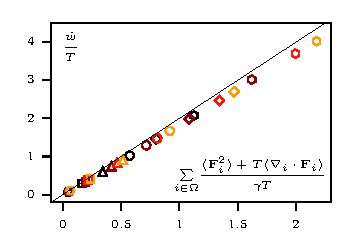
\includegraphics[width=\linewidth]{fig1.pdf}
	\caption{\label{fig:fig1}
		Parametric plot of the rate of work $\dot w/T$ and the statistics of bath-tracer forces $\sum_{i\in\Omega}\big[\langle{\bf F}_i^2\rangle + T\langle\nabla_i\cdot{\bf F}_i\rangle\big]/\gamma T$, where the sum runs over driven tracer particles, for a dilute fraction of driven particles ($10\%$). $\tau/\tau_{\rm r}=20$ (black), $30$ (brown), $40$ (red), $50$ (orange). ${\rm Pe}=6$ ($\hexagon$), $12$ ($\boxempty$), $18$ ({\large$\vartriangle$}), $24$ ({$\Circle$}), $30$ (${\Diamond}$), $36$ ($\varhexagon$). The good agreement with the approximate relation~\eqref{eq:approx}, in solid line, indicates that dissipation can be estimated by only measuring bath-tracer forces.
		Simulation details in Appendix~\ref{app:simu}.
	}
\end{figure}


To further evaluate the change in liquid structure induced by dissipation, we measure the deviation from equilibrium pair-correlation $g-g_{\rm eq}$ due to the driving forces. At a given $\tau/\tau_{\rm r}$, scaling ${\cal I} = \big[(\nabla v)^2-T\nabla^2v\big](g - g_{\rm eq})$ by ${\rm Pe}^2$ reveals that all curves almost collapse into a master curve for our numerical range ${\rm Pe}\in[12,36]$, as shown in the middle column of Fig.~\ref{fig:fig2}. Given that the rate of work also exhibits such a scaling, this suggests the existence of an underlying relation between $\int{\cal I}({\bf r}){\rm d}{\bf r}$ and $\dot w$: it appears that their ratio indeed gives a factor close to $\rho_0/\gamma$, as depicted in the right column of Fig.~\ref{fig:fig2}. Hence, this empirical relation shows that, considering the periodic drive~\eqref{eq:theta} in the dilute limit, the dissipation can be directly estimated by comparing driven and equilibrium pair-correlations: this is clearly an asset with respect to invasive methods based on comparing fluctuations and response~\cite{Harada2005, Mizuno2007, Visco2015, Turlier2016, Ahmed2018}.


\begin{figure*}
	\centering
	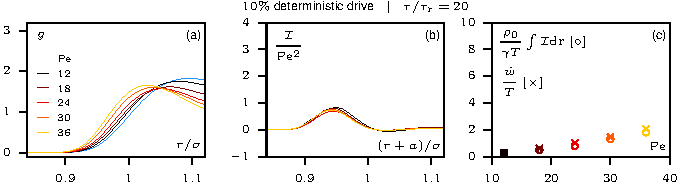
\includegraphics[width=\linewidth]{fig2a.pdf}
	\vskip.5cm
	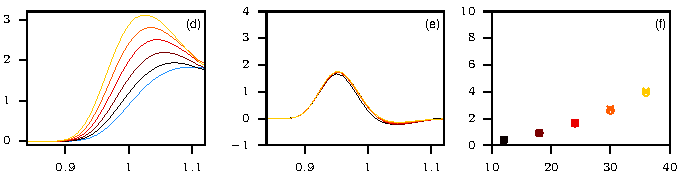
\includegraphics[width=\linewidth]{fig2b.pdf}
	\vskip.5cm
	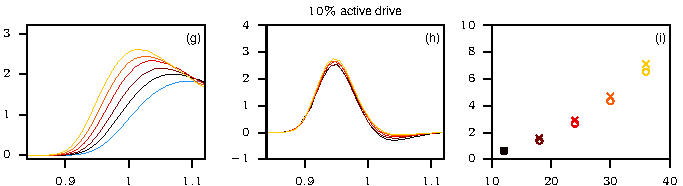
\includegraphics[width=\linewidth]{fig2c.pdf}
	\vskip.5cm
	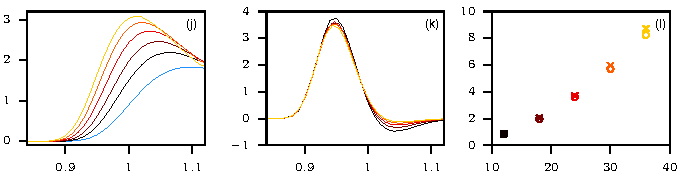
\includegraphics[width=\linewidth]{fig2d.pdf}
	\caption{\label{fig:fig2}
		(Left) Bath-tracer density correlation $g$ as a function of inter-particle distance $r/\sigma$. Blue solid line is equilibrium correlation $g_{\rm eq}$ for ${\rm Pe}=0$.
		(Middle) ${\cal I} = \big[(\nabla v)^2-T\nabla^2v\big](g - g_{\rm eq})$ scaled by ${\rm Pe}^2$ as a function of $r/\sigma$. For a given $\tau/\tau_{\rm r}$, the data almost collapse into a master curve.
		(Right) $(\rho_0/\gamma T)\int{\cal I}({\bf r}){\rm d}{\bf r}$ and rate of work $\dot w/T$ as functions of $\rm Pe$. The former under-estimates $\dot w$ by at most approximately $10\%$, showing that deviation from equilibrium pair correlations provides a direct access to dissipation with only a small error.
		Simulation details in Appendix~\ref{app:simu}.
	}
\end{figure*}


Overall, the results of this Section illustrate how dissipation affects the transport properties of a driven liquid, measured in terms of diffusion coefficient, as well as its structural properties, characterized by density fluctuations. This immediately suggests that internal transport and emerging structure can be tuned externally by monitoring the nonequilibrium forces which power the dissipation. A related question then is whether specific structures and correlations can be stabilized by biasing particle trajectories which pump energy into or out of specific interactions. As mentioned previously, we regard such a bias as a way to mimic the effect of generic external drive. We now investigate this question. 


% ===============================================================================


\section{Interactions in biased ensembles}\label{sec:bias}

To explore how energy flows affect the microscopic interactions, we consider biasing the dynamics in terms of the rate of energy stored in the pair potential energy between specific subsets of particles. To sample such a {\it biased ensemble}, we rely on the framework of large deviation theory~\cite{Chetrite2013, Jack2010}. Formally, the biased ensemble is generated by introducing a weighting factor $\exp\big[\kappa\int_0^t{\cal E}(s){\rm d}s\big]$ in the dynamical path probability. The trajectories and configurations in biased ensemble are then associated with a given statistics of $\cal E$, which can be tuned by monitoring $\kappa$. Such trajectory biases have already been used in a large variety of contexts, for instance, to explore dynamical heterogeneities in glassy systems~\cite{garrahan2007, Hedges2009, Pitard2011, Speck2012, Bodineau2012a, Limmer2014, Nemoto2017}, soliton solutions in high-dimensional chaotic chains~\cite{tailleur2007probing, laffargue2013} and, more recently, the clustering of self-propelled particles~\cite{Cagnetta2017, Whitelam2018, nemoto2018optimizing}.


In what follows, we consider the effect of biasing the dynamics with $\varepsilon(t)=\sum_{i,j} \kappa_{ij}\int_0^t{\cal E}_{ij}(s){\rm d}s$ where 
\begin{equation}\label{eq:eps}
	{\cal E}_{ij} = \frac{1}{2\gamma T}\sum_k\big[ \delta_{k\in\Omega}{\bf F}_{\rm d} - \nabla_k V + T \nabla_k\big] \cdot\nabla_k v({\bf r}_i-{\bf r}_j) ,
\end{equation}
and $V=(1/2)\sum_{i,j}v({\bf r}_i-{\bf r}_j)$. The control parameters $\kappa_{ij}$ are specific for any given pair of particles $\{i\,,j\}$. They can be chosen so that the rate of change of only specific inter-particle pair potentials are accounted for and used for biasing. Indeed, with the definition~\eqref{eq:eps}, we get $2T\langle{\cal E}_{ij}\rangle_\varepsilon = \langle\dot v({\bf r}_i-{\bf r}_j)\rangle_\varepsilon$, where $\langle\cdot\rangle_\varepsilon=\big\langle\cdot\,{\rm e}^\varepsilon\big\rangle\big/\big\langle{\rm e}^\varepsilon\big\rangle$ denotes here an average in the biased ensemble. In the unbiased case ($\kappa_{ij}=0$), there are no energy flows for any pair of particles, so that $\langle\dot v\rangle_\varepsilon = 0$. At variance, by tuning $\kappa_{ij}$ positive (negative), one can now generate trajectories that preferentially inject (extract) energy into (from) some specific interactions by effectively realizing $\langle\dot v\rangle_\varepsilon>0$ ($\langle\dot v\rangle_\varepsilon<0$).


Following the procedure in~\cite{Chetrite2013}, an auxiliary physical dynamics, with the same statistical properties as in the biased ensemble, can be constructed by solving the following eigenvalue equation 
\begin{equation}\label{eq:adjointbiased}
	\Big[L^\dagger + \sum_{i,j}\kappa_{ij}{\cal E}_{ij}\Big]\,{\cal G}({\bf r}_k,\kappa) = \lambda(\kappa)\,{\cal G}({\bf r}_k,\kappa) ,
\end{equation}
where the eigenvalue $\lambda$, parametrized by $\kappa_{ij}$, is the scaled cumulant generating function appropriate to the biasing observable $\varepsilon$. The operator $L^\dagger$ is the adjoint of the Fokker-Planck operator associated with the dynamics~\eqref{eq:dyn}:
\begin{equation}\label{eq:L}
	L^\dagger = \frac{1}{\gamma} \sum_i\big[ \delta_{i\in\Omega}{\bf F}_{\rm d} - \nabla_i V + T \nabla_i\big] \cdot\nabla_i .
\end{equation}
The force field $\tilde{\bf F}_i$ of the auxiliary dynamics is then defined in terms of the eigenfunction ${\cal G}$ as 
\begin{equation}
	\tilde{\bf F}_i = \delta_{i\in\Omega}{\bf F}_{\rm d} - \nabla_iV + 2 T \nabla_i \ln{\cal G} .
\end{equation}
In practice, computing $\tilde {\bf F}_i$ is a highly non-trivial procedure for many-body systems, the explicit solutions obtained so far are only either perturbative or restricted to non-interacting systems~\cite{Chetrite2013, Touchette2016}.


In our case, a simple expression can be obtained for the auxiliary force $\tilde{\bf F}_i$  by solving~\eqref{eq:adjointbiased} perturbatively in terms of the bias parameter $\kappa_{ij}$. Specifically, we expand
\begin{equation}
	\begin{aligned}
		\lambda(\kappa) &= \frac{1}{2T} \sum_{i,j}\kappa_{ij}\langle\dot v({\bf r}_i- {\bf r}_j)\rangle + {\cal O}(\kappa^2) ,
		\\
		{\cal G}({\bf r}_k,\kappa) &= {\cal G}^{(0)} + \sum_{i,j}\kappa_{ij}{\cal G}_{ij}^{(1)}({\bf r}_k) + {\cal O}(\kappa^2) ,
	\end{aligned}
\end{equation}
where $\langle\cdot\rangle$ is the average in the unbiased case, and ${\cal G}^{(0)}$ is the uniform eigenvector associated with the zero eigenvalue. Given that $\langle\dot v\rangle=0$ in steady state, the leading non-trivial order of~\eqref{eq:adjointbiased} reads
\begin{equation}
	\sum_{i,j}\kappa_{ij}\Big[L^\dagger{\cal G}_{ij}^{(1)} + {\cal G}^{(0)} {\cal E}_{ij}\Big] + {\cal O}(\kappa^2) = 0 .
\end{equation}
Substituting the explicit expressions for the biasing function~\eqref{eq:eps} and for the operator~\eqref{eq:L}, we then deduce that $2T{\cal G}_{ij}^{(1)}=-{\cal G}^{(0)} v({\bf r}_i-{\bf r}_j)$ is a solution of the eigenvalue problem to order $\kappa_{ij}$. The auxiliary force follows as
\begin{equation}\label{eq:F}
	\tilde{\bf F}_k = \delta_{k\in\Omega}{\bf F}_{\rm d} - \frac{1}{2}\nabla_k\sum_{i,j}(1+2\kappa_{ij}) v({\bf r}_i-{\bf r}_j) + {\cal O}(\kappa^2) .
\end{equation}
As a result, the trajectories that extract (inject) energy from (into) some pair interactions can be generated with a physical dynamics where interactions are simply renormalized, at leading order, with a specific strength $1+2\kappa_{ij}$ for each pair. For systems with purely repulsive pairwise interactions, modifying the interaction strength between targeted particle pairs is qualitatively consistent with the effect of external driving. For instance, phase separation in mixtures of driven and undriven particles, reported both experimentally and numerically~\cite{delJunco2018,Han2016}, can be rationalized in terms of an effective decrease of specific interactions between these particles.


Moreover, the effect of higher order bias can be anticipated by considering another biasing observable:
\begin{equation}\label{eq:eps_prime}
	\varepsilon' = \frac{1}{4\gamma T}\int_0^t\sum_k\Big[\sum_{i,j}\kappa_{ij}\nabla_kv({\bf r}_i(s)-{\bf r}_j(s))\Big]^2{\rm d}s .
\end{equation}
As shown in Appendix~\ref{sec:far}, biasing the original dynamics~\eqref{eq:dyn} with $\varepsilon$ is equivalent to biasing the auxiliary dynamics, specified by~\eqref{eq:F}, with $\varepsilon'$. In short, the original bias then results in two combined effects: (i) modifying some specific pair potentials, and (ii) optimizing the total squared force in the integrand of $\varepsilon'$, which effectively tends to cluster particles.


To probe the range of validity of our perturbation, we consider an assembly of passive Brownian particles ($|{\bf F}_{\rm d}|=0$) where all the pairs between a subset $\Omega$ and other particles are biased with the same strength $\kappa$, such as $\kappa_{ij}=\kappa\delta_{i\in\Omega}\delta_{j\not\in\Omega}$. To make connection with the setup used in the previous Sections, $\Omega$ could for instance be the set of tracer particles. With this choice, we get $2T\sum_{i,j}\kappa_{ij}\langle{\cal E}_{ij}\rangle_\varepsilon = \kappa\langle\dot U\rangle_\varepsilon$ where $U = \sum_{i\in\Omega,j\not\in\Omega} v({\bf r}_i-{\bf r}_j)$. In other words, we are biasing the flow of energy into bonds between particles in the subset $\Omega$ and all other particles. 


\begin{figure*}
	\centering
	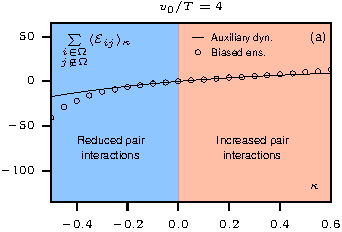
\includegraphics[width=.49\linewidth]{fig3a.pdf}
	\hfill
	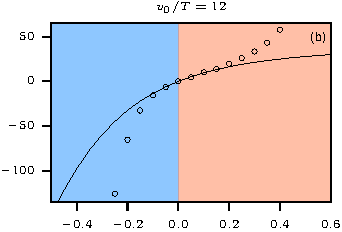
\includegraphics[width=.49\linewidth]{fig3b.pdf}
	\vskip.5cm
	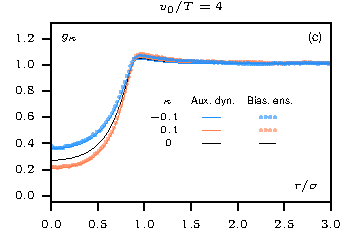
\includegraphics[width=.49\linewidth]{fig3c.pdf}
	\hfill
	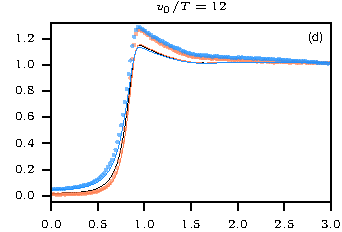
\includegraphics[width=.49\linewidth]{fig3d.pdf}
	\caption{\label{fig:energybias}
		(a-b)~Average rate of biased potential energy $\langle\dot U\rangle_\varepsilon/T$ as a function of bias parameter $\kappa$: auxiliary dynamics and direct sampling of the biased ensemble respectively in circles and solid lines.
		(c-d)~Biased density correlation $g_\varepsilon$ as a function of inter-particle distance $r/\sigma$: auxiliary dynamics and direct sampling respectively in solid and dotted lines.
		Biasing modifies the total pair potential $U$ by a factor $\kappa$ at leading order. The good agreement between auxiliary dynamics and direct sampling illustrates the control of liquid structure at small $\kappa$.
		Simulation details in Appendix~\ref{app:simu}.
}
\end{figure*}


We compare measurements of $\langle\dot U\rangle_\varepsilon$ obtained from simulations of the auxiliary dynamics~\eqref{eq:F} and from a direct sampling of the biased ensemble. The latter is implemented with a cloning algorithm where rare realizations are regularly selected and multiplied for efficient sampling~\cite{Giadina2006, tailleur2007probing, Hurtado2009, Nemoto2016, Ray2018, Klymko2018, Brewer2018}. For convenience, interactions are now given by the soft-core potential $v({\bf r}) = v_0\exp\big[-1 / (1 - (|{\bf r}|/\sigma)^2)\big]\Theta(\sigma-|{\bf r}|)$. We observe a very good agreement between the two measurements for a range of $\kappa$. In particular, the agreement improves as $v_0/T$ is decreased, as reported in Figs.~\ref{fig:energybias}(a-b). This supports the validity of our perturbation in this regime, up to interaction change of about $+40\%$ when $v_0/T=4$. Note that the range of validity is asymmetric in $\kappa$.


To explore further the features of the biased ensemble, we now compare the density correlations of biased pairs $g_\varepsilon({\bf r})=(1/N) \sum_{i\in\Omega,j\not\in\Omega}\langle \delta({\bf r}-{\bf r}_i+{\bf r}_j)\rangle_\varepsilon$ obtained from both direct sampling and auxiliary dynamics. At $\kappa=\pm0.1$, the agreement is good for the whole curve when $v_0/T=4$, whereas a clear deviation appears beyond $r\simeq\sigma$ when $v_0/T=12$, as shown in Figs.~\ref{fig:energybias}(c-d). In both cases, the region of particle overlap $r<\sigma$ is well reproduced, as expected, since it is entirely controlled by the interaction change captured in~\eqref{eq:F}. Yet, the tendency for particles to cluster, manifest in the peak at $r\simeq\sigma$, comes as a higher order effect beyond this perturbation. Note that the peak value is comparable for $\kappa=\pm0.1$, in agreement with~\eqref{eq:eps_prime} being symmetric in $\kappa$. Besides, at fixed $\kappa$, the structural modification becomes more dramatic as $v_0/T$ increases. Altogether, these results demonstrate that selecting trajectories which preferentially inject (extract) energy into (from) some specific pair interactions, by tuning $\kappa$, indeed modulates the liquid structure in a controlled manner for small bias and weak interactions.


\begin{figure*}
	\centering
	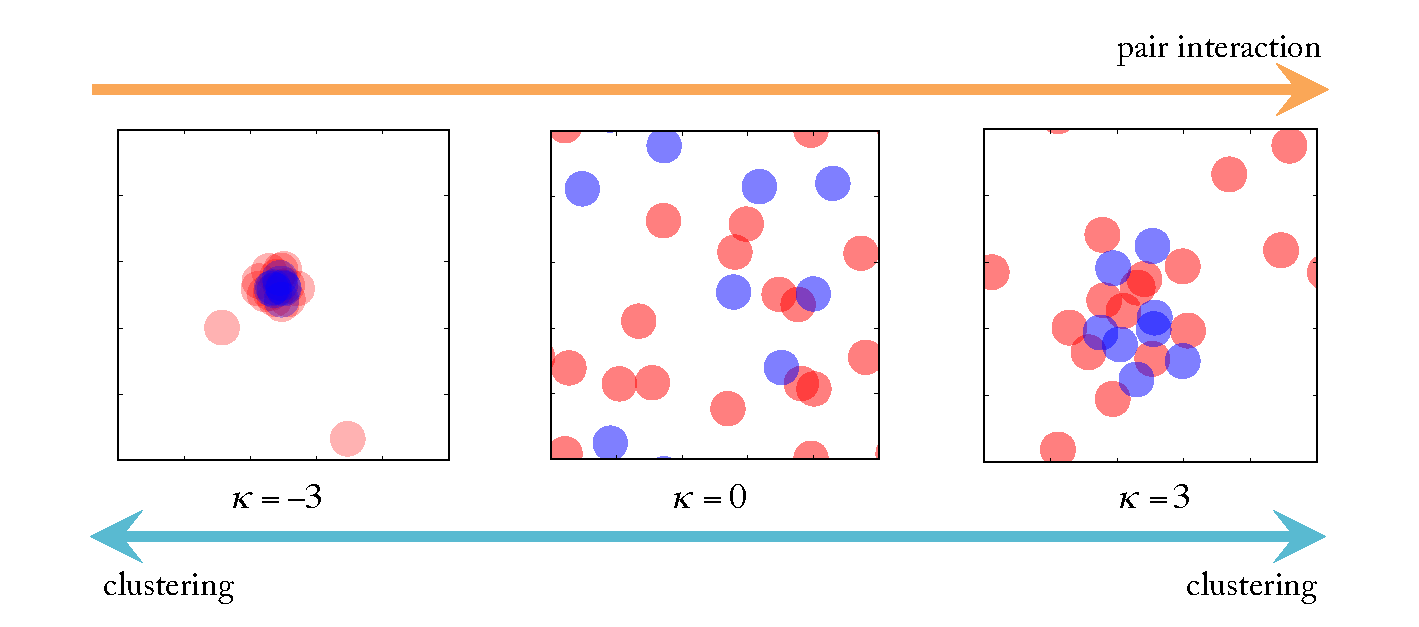
\includegraphics[width=.8\linewidth]{fig4.pdf}
	\caption{\label{fig:outofperturbation}
	Configurations in biased ensemble obtained from direct sampling: biased pair potentials are the ones between blue and red particles. Blue and orange arrows respectively indicate (i) the increased propensity to form clusters for $\kappa=\pm3$, and (ii) the increase of pair interactions from $\kappa=-3$ to $3$. As a result, particles aggregate either with a random composition ($\kappa=3$) or in a micelle-like structure with a blue core ($\kappa=-3$), showing that pair interaction bias can favor some selected structures.
		Simulation details in Appendix~\ref{app:simu}.
	}
\end{figure*}


Finally, to determine whether our bias can stabilize configurations which are significantly distinct from the unbiased system, we probe numerically the effect of large bias $|\kappa|>1$ from direct sampling. The particles spontaneously tend to cluster for both positive and negative $\kappa$, as shown in Fig.~\ref{fig:outofperturbation}. This confirms the propensity of trajectories to maximize interaction forces at high bias, in agreement with~\eqref{eq:eps_prime}. The shape of clusters differs depending on the sign of $\kappa$: a micelle-like structure featuring the particles in $\Omega$ at the core (blue) surrounded by others (red) appears for $\kappa=-3$, whereas clusters have a random composition for $\kappa=3$. Again, this agrees with~\eqref{eq:F}, where the interactions strength is either increased or decreased, respectively for $\kappa>0$ and $\kappa<0$. Overall, these results establish a reliable proof of principle for the design of self-assembled structures based on biasing energy flows into or out of particular pair interactions.


% ===============================================================================


\section{Conclusion}

Developing techniques to characterize and control the behavior of systems operating far from equilibrium remains a central and outstanding problem. In this paper, we have demonstrated that specifying the amount of energy dissipated by nonequilibrium forces allows one to constrain the dynamics and structure of such systems. Despite the apparently complex interplay between internal dissipation and emerging properties, their exist simple connections between tracer diffusion, density correlations and dissipation in a driven liquid. It remains to investigate whether similar results can be obtained in more complex systems, for instance including anisotropic building blocks, such as active liquid crystals or driven chiral objects~\cite{Joshi2017, VanZuiden2016, Nguyen2014b}.


Motivated by these findings, we have also put forward a novel method to control  liquid structure: it relies on biasing the dynamics with the pair potential between individual components. For a minimal case study, we have shown that the emerging biased configurations, sampled with state-of-the-art numerics~\cite{Giadina2006, tailleur2007probing, Hurtado2009, Nemoto2016, Ray2018, Klymko2018, Brewer2018}, could be rationalized using recent methods of large deviation theory~\cite{Chetrite2013, Jack2010}. Importantly, since our analytic results encompass the case of a specific bias for each pair, it might be possible to promote the spontaneous self-assembly of more complex structures in such biased ensembles. For instance, inspired by recent works~\cite{Murugan2015, Murugan2017b}, one could potentially design appropriate energetic landscapes, in terms of the pair-specific bias parameters, to selectively stabilize some target molecules. Finally, our results extend straightforwardly to active systems~\cite{Marchetti2013, Cates2015, Bechinger2016, Marchetti2018}, where the driving force has now an independent dynamics for each particle, opening the door to control self-organization in biological context~\cite{Sperandio2002, Brown2011, Betz2018}.


% ===============================================================================


\acknowledgements{This work was granted access to the HPC resources of CINES/TGCC under the allocation 2018-A0042A10457 made by GENCI and of MesoPSL financed by the Region Ile de France and the project Equip@Meso (reference ANR-10-EQPX-29-01) of the program Investissements d'Avenir supervised by the Agence Nationale pour la Recherche.
SV and LT were supported by the University of Chicago Materials Research Science and Engineering Center, which is funded by National Science Foundation under award number DMR-1420709. SV acknowledges support from the Sloan Foundation and startup funds from the University of Chicago. \'EF benefits from an Oppenheimer Research Fellowship from the University of Cambridge, and a Junior Research Fellowship from St Catherine's College.}


% ===============================================================================


\appendix

\section{Dissipation and diffusion}\label{app:diff}

This appendix is devoted to the derivation of the dissipation rate $\cal J$ and the diffusion coefficient $D$ of a driven tracer, as defined in Sec.~\ref{sec:method}. We employ a perturbative treatment at weak interactions, originally introduced for a particle driven at constant force in~\cite{Demery2011, Demery2014}. To this aim, the tracer-bath interaction potential $v$ is scaled by a small dimensionless parameter $h\ll1$ in what follows. Besides, we focus on the regime of dilute tracers, so that interactions among them, either direct or mediated by the bath, can be safely neglected .


The dynamic action associated with the tracer dynamics~(\ref{eq:rho}-\ref{eq:EvolutionTracer}) follows from standard path integral methods~\cite{Martin1973, Dominicis1975}. It can be separated into contributions from the free tracer motion and from interactions, respectively denoted by ${\cal A}_0$ and ${\cal A}_{\rm int}$:
\begin{equation}\label{eq:action}
	\begin{aligned}
		{\cal A}_0 &= \int \bar{\bf r}_0 \cdot \big[ {\rm i}(\dot{\bf r}_0 - {\bf F}_{\rm d}/\gamma) + D_0 \bar{\bf r}_0 \big] {\rm d}t ,
		\\
		{\cal A}_{\rm int} &= h^2 \int \frac{{\rm d}{\bf q}}{(2\pi)^d} |{\bf q}|^2 |v({\bf q})|^2 \int_{-\infty}^\infty {\rm d}s\int_{-\infty}^s{\rm d}u
		\\
		&\quad\times {\rm e}^{-D_{\rm G}|{\bf q}|^2K({\bf q})(s-u)+{\rm i}{\bf q}\cdot[{\bf r}_0(s)-{\bf r}_0(u)]}
		\\
		&\quad\times \bar{\bf r}_0(s) \cdot \bigg[ \frac{\bar{\bf r}_0(u)}{K({\bf q})} - \frac{{\bf q}}{\gamma_{\rm G}} \bigg] ,
	\end{aligned}
\end{equation}
where $D_0=T/\gamma$ is the tracer diffusion coefficient in the absence of interactions ($v=0$), and $\bar{\bf r}_0$ is the process conjugated with the tracer position ${\bf r}_0$. For weak interactions $h\ll1$, any average value can be then expanded in terms of $h$ as $\langle\cdot\rangle=\langle\cdot\rangle_0 - h^2 \langle{\cal A}_{\rm int}\cdot\rangle_0 + {\cal O}(h^4)$, where $\langle\cdot\rangle_0$ is the average taken with respect to ${\cal A}_0$ only. As a result, determining the first correction from interactions in any observable amounts to computing the corresponding average $\langle{\cal A}_{\rm int}\cdot\rangle_0$.


Considering the dissipation rate ${\cal J}=\langle\dot{\bf r}_0\rangle\cdot{\bf F}_{\rm d}$, the leading order is $\langle\dot{\bf r}_0\rangle_0 \cdot {\bf F}_{\rm d} = |{\bf F}_{\rm d}|^2/\gamma = f^2/\gamma$, and the first correction reads $ - h^2 \langle{\cal A}_{\rm int}\dot{\bf r}_0\rangle_0 \cdot {\bf F}_{\rm d} $. Given the explicit form of ${\cal A}_{\rm int}$ in~\eqref{eq:action}, the correlations of interest are
\begin{equation}
	\begin{aligned}
		\Big\langle\dot{\bf r}_0(t) &\big[{\bf q}\cdot\bar{\bf r}_0(s)\big] {\rm e}^{{\rm i}{\bf q}\cdot[{\bf r}_0(s)-{\bf r}_0(u)]}\Big\rangle_0
		\\
		&= \frac{{\rm i}{\bf q}}{\gamma}\delta(t-s){\rm e}^{ - D_0|{\bf q}|^2(t-u) + \frac{{\rm i}{\bf q}}{\gamma}\cdot\int_u^t {\bf F}_{\rm d}(w) {\rm d}w} ,
		\\
		\Big\langle\dot{\bf r}_0(t) &\big[\bar{\bf r}_0(u)\cdot\bar{\bf r}_0(s)\big] {\rm e}^{{\rm i}{\bf q}\cdot[{\bf r}_0(s)-{\bf r}_0(u)]}\Big\rangle_0
		\\
		&= -\frac{{\rm i}{\bf q}}{\gamma^2}\delta(t-s){\rm e}^{ - D_0|{\bf q}|^2(t-u) + \frac{{\rm i}{\bf q}}{\gamma}\cdot\int_u^t {\bf F}_{\rm d}(w) {\rm d}w} ,
	\end{aligned}
\end{equation}
where we have used that the tracer statistics is Gaussian in the absence of interactions, following~\cite{Demery2011, Demery2014}. From this result, we get
\begin{equation}
	\begin{aligned}
		&{\cal J} - f^2/\gamma
		\\
		&\,= \frac{h^2}{d\gamma^2} \int \frac{{\rm d}{\bf q}}{(2\pi)^d} {\rm i}{\bf q}\cdot{\bf F}_{\rm d}(t) |{\bf q}|^2 |v({\bf q})|^2 \frac{D_0+D_{\rm G}K({\bf q})}{D_0K({\bf q})}
		\\
		&\,\quad\times \int_{-\infty}^t {\rm d}u {\rm e}^{-|{\bf q}|^2 [D_0+D_{\rm G} K({\bf q})](t-u) + \frac{{\rm i}{\bf q}}{\gamma}\cdot\int_u^t{\bf F}_{\rm d}(w){\rm d}w}
		\\
		&\,\quad + {\cal O}(h^4) ,
	\end{aligned}
\end{equation}
where we have used $\gamma_{\rm G}=\gamma/\rho_0$ and $D_{\rm G}=\rho_0D_0$. Expanding at small $f$, we deduce
\begin{equation}
	\begin{aligned}
		&{\cal J} - f^2/\gamma
		\\
		&\,= - \frac{h^2}{d\gamma^3} \int \frac{{\rm d}{\bf q}}{(2\pi)^d} |{\bf q}|^4 |v({\bf q})|^2 \frac{D_0+D_{\rm G}K({\bf q})}{D_0K({\bf q})}
		\\
		&\,\quad\times \int_{-\infty}^t {\rm d}u {\rm e}^{-|{\bf q}|^2 [D_0+D_{\rm G} K({\bf q})](t-u)} \int_u^t{\rm d}w{\bf F}_{\rm d}(t)\cdot{\bf F}_{\rm d}(w)
		\\
		&\,\quad + {\cal O}(h^4,f^4) .
	\end{aligned}
\end{equation}
Substituting the explicit expression of the drive~\eqref{eq:theta}, and integrating over $u$ and $w$, we obtain
\begin{equation}
	\begin{aligned}
		{\cal J} - \frac{f^2}{\gamma} &= - \frac{(hf)^2}{d\gamma^3} \int \frac{{\rm d}{\bf q}}{(2\pi)^d} \frac{|{\bf q}|^4 |v({\bf q})|^2}{|{\bf q}|^4\big[D_0+D_{\rm G}K({\bf q})\big]^2 + \omega^2}
		\\
		&\quad\times \frac{D_0+D_{\rm G}K({\bf q})}{D_0K({\bf q})} + {\cal O}(h^4,f^4) .
	\end{aligned}
\end{equation}
The asymptotic results for the rate of work $\dot w = f^2/\gamma-{\cal J}$ in~(\ref{eq:small}-\ref{eq:large}) follow directly.


We now turn to deriving the diffusion coefficient $D$. It is defined in terms of the mean-squared displacement (MSD) $\langle\Delta{\bf r}_0^2(t)\rangle=\big\langle\big[\langle{\bf r}_0(t)\rangle - {\bf r}_0(t)\big]^2\big\rangle$ as $D=\underset{t\to\infty}{\lim}\langle\Delta{\bf r}_0^2(t)\rangle / 2 d t$. At leading order, the MSD reads $\langle\Delta{\bf r}_0^2(t)\rangle_0 = 2dD_0t$. To obtain the first order, we need to compute the following correlations
\begin{equation}
	\begin{aligned}
		\Big\langle\Delta{\bf r}^2_0(t)& \big[{\bf q}\cdot\bar{\bf r}_0(s)\big] {\rm e}^{{\rm i}{\bf q}\cdot[{\bf r}_0(s)-{\bf r}_0(u)]}\Big\rangle_0
		\\
		&= - 4 (D_0/\gamma)|{\bf q}|^2(s-u) \Theta(t-s)
		\\
		&\quad\times{\rm e}^{ - D_0|{\bf q}|^2(t-u) + \frac{{\rm i}{\bf q}}{\gamma}\cdot\int_u^t {\bf F}_{\rm d}(w) {\rm d}w},
		\\
		\Big\langle\Delta{\bf r}^2_0(t)& \big[\bar{\bf r}_0(u)\cdot\bar{\bf r}_0(s)\big] {\rm e}^{{\rm i}{\bf q}\cdot[{\bf r}_0(s)-{\bf r}_0(u)]}\Big\rangle_0
		\\
		&= (2/\gamma^2)\Theta(t-s) \big[2D_0|{\bf q}|^2(s-u)-1\big]
		\\
		&\quad\times{\rm e}^{ - D_0|{\bf q}|^2(t-u) + \frac{{\rm i}{\bf q}}{\gamma}\cdot\int_u^t {\bf F}_{\rm d}(w) {\rm d}w} ,
	\end{aligned}
\end{equation}
where we have used again that ${\cal A}_0$ is Gaussian in terms of $\bar{\bf r}_0$, yielding
\begin{equation}
	\begin{aligned}
		&\big\langle\Delta{\bf r}^2_0(t)\big\rangle - 2 d D_0 t
		\\
		&\,= \frac{2h^2}{\gamma^2} \int \frac{{\rm d}{\bf q}}{(2\pi)^d} \frac{|{\bf q}|^2 |v({\bf q})|^2}{K({\bf q})}
		\\
		&\,\quad\times \int_{-\infty}^t{\rm d}s \int_{-\infty}^s{\rm d}u \big\{ 2|{\bf q}|^2\big[D_0+D_{\rm G}K({\bf q})\big](s-u) - 1\big\}
		\\
		&\,\quad\times {\rm e}^{ -|{\bf q}|^2[D_0+D_{\rm G}K({\bf q})](s-u) + \frac{{\rm i}{\bf q}}{\gamma}\cdot\int_u^s{\bf F}_{\rm d}(w) {\rm d}w } + {\cal O}(h^4) .
	\end{aligned}
\end{equation}
Expanding at small $f$, we get
\begin{equation}
	\begin{aligned}
		&\big\langle\Delta{\bf r}^2_0(t)\big\rangle - 2 d D_{\rm eq} t
		\\
		&\,= - \frac{2h^2}{\gamma^4} \int \frac{{\rm d}{\bf q}}{(2\pi)^d} \frac{|{\bf q}|^4 |v({\bf q})|^2}{K({\bf q})}
		\\
		&\,\quad\times \int_{-\infty}^t{\rm d}s \int_{-\infty}^s{\rm d}u \big\{ 2|{\bf q}|^2\big[D_0+D_{\rm G}K({\bf q})\big](s-u) - 1\big\}
		\\
		&\,\quad\times {\rm e}^{ -|{\bf q}|^2[D_0+D_{\rm G}K({\bf q})](s-u)} \int_u^s {\rm d}w_1{\rm d}w_2 {\bf F}_{\rm d}(w_1)\cdot{\bf F}_{\rm d}(w_2)
		\\
		&\,\quad + {\cal O}(h^4,f^4) ,
	\end{aligned}
\end{equation}
where $D_{\rm eq}$ refers to the diffusion coefficient in the absence of driving force ($f=0$). From the explicit time integrations, we then obtain
\begin{equation}
	\begin{aligned}
		D - D_{\rm eq} &= \frac{(hf)^2}{d\gamma^4} \int \frac{{\rm d}{\bf q}}{(2\pi)^d} \frac{|{\bf q}|^2|v({\bf q})|^2}{K({\bf q})\big[D_0+D_{\rm G}K({\bf q})\big]}
		\\
		&\quad\times \frac{5|{\bf q}|^4\big[D_0+D_{\rm G}K({\bf q})\big]^2 + \omega^2}{ \big\{ |{\bf q}|^4\big[D_0+D_{\rm G}K({\bf q})\big]^2 + \omega^2 \big\}^2}
		\\
		&\quad + {\cal O}(h^4,f^4)  .
	\end{aligned}
\end{equation}
Finally, we deduce the corresponding expressions in the asymptotic regimes in~(\ref{eq:small}-\ref{eq:large}).


% -------------------------------------------------------------------------------


\section{Numerical simulations}\label{app:simu}

In Sec.~\ref{sec:method}, numerical simulations of the dynamics~\eqref{eq:dyn} are performed using the LAMMPS simulation package in a two-dimensional box $10^2\sigma\times 10^2\sigma$, where $\sigma$ is the particle diameter, with periodic boundary conditions at average density $\rho_0=0.45$. The driving force ${\bf F}_{\rm d}$ only acts on ten percent of the particles with dynamics~\eqref{eq:theta}. The time step is $\delta t = 5\times 10^{-4} \tau_{\rm r}$. The system is first relaxed for $10^5$ time steps, and later equilibrated for $50\tau$. We evaluate average values over trajectories with duration of at least $150\tau$. Parameter values: $T=1$, $\gamma=10^2$, $v_0=1$, $\sigma=1$.


In Sec.~\ref{sec:bias}, a custom code of molecular dynamics, based on finite time difference, is used to perform the simulations in a two-dimensional box $10\sigma\times 10\sigma$ with periodic boundary conditions. The pair potential of $16$ particle pairs is biased in a system of $40$ particles in total. To sample the biased ensemble, we use the cloning algorithm described in Appendix A of~\cite{Nemoto2016}. The time interval for cloning is $\Delta t = 10 \delta t$ and the number of clones is $1600$. The time step is $\delta t = 10^{-4} \tau_{\rm r}$, the initial relaxation time is $10^4\Delta t$, and the total simulation time is $10^6 \Delta t$. Parameter values: $T=1$, $\gamma=1$, $v_0=4$ (Fig.~\ref{fig:outofperturbation}), $\sigma=1$.


% -------------------------------------------------------------------------------


\begin{widetext}
\section{Equivalence of biased ensembles}\label{sec:far}

In this Appendix, we demonstrate the equivalence between two dynamical biased ensembles: (i) the original dynamics~\eqref{eq:dyn} biased with $\varepsilon(t)=\sum_{i,j} \kappa_{ij}\int_0^t{\cal E}_{ij}(s){\rm d}s$, where ${\cal E}_{ij}$ is defined in~\eqref{eq:eps}, and (ii) the auxiliary dynamics with force field~\eqref{eq:F} biased with $\varepsilon'$ defined in~\eqref{eq:eps_prime}. This amounts to showing that the path probabilities associated with (i) and (ii) are similar. The corresponding dynamic actions, respectively denoted by ${\cal A}^{(\rm i)}(t)=\sum_k\int_0^t{\cal L}_k^{(\rm i)}(s){\rm d}s$ and ${\cal A}^{(\rm ii)}(t)=\sum_k\int_0^t{\cal L}_k^{(\rm ii)}(s){\rm d}s$, are given here in terms of the Lagragians ${\cal L}_k^{(\rm i)}$ and ${\cal L}_k^{(\rm ii)}$ defined as
\begin{equation}\label{eq:lag}
	\begin{aligned}
		{\cal L}_k^{(\rm i)} &= \frac{1}{4\gamma T} \bigg[\gamma\dot{\bf r}_k - \delta_{k\in\Omega}{\bf F}_{\rm d} + \frac{1}{2}\nabla_k\sum_{i,j}v({\bf r}_i-{\bf r}_j)\bigg]^2 - \frac{1}{4\gamma} \sum_{i,j}\nabla^2_kv({\bf r}_i-{\bf r}_j)
		\\
		&\quad - \frac{1}{2\gamma T} \sum_{i,j}\kappa_{ij}\big[\delta_{k\in\Omega}{\bf F}_{\rm d} - \nabla_k V + T \nabla_k\big] \cdot\nabla_k v({\bf r}_i-{\bf r}_j) ,
		\\
		{\cal L}_k^{(\rm ii)}	&= \frac{1}{4\gamma T} \bigg[\gamma\dot{\bf r}_k - \delta_{k\in\Omega}{\bf F}_{\rm d} + \frac{1}{2}\nabla_k\sum_{i,j}(1+2\kappa_{ij})v({\bf r}_i-{\bf r}_j)\bigg]^2 - \frac{1}{4\gamma} \sum_{i,j}(1+2\kappa_{ij})\nabla^2_kv({\bf r}_i-{\bf r}_j)
		\\
		&\quad - \frac{1}{4\gamma T}\Big[\sum_{i,j}\kappa_{ij}\nabla_kv({\bf r}_i-{\bf r}_j)\Big]^2 .
	\end{aligned}
\end{equation}
Expanding ${\cal L}_k^{(\rm i)}$ and ${\cal L}_k^{(\rm ii)}$, it appears that ${\cal A}^{(\rm i)}$ and  ${\cal A}^{(\rm ii)}$ are indeed equal, up to a boundary term proportional to $\sum_{i,j}\kappa_{ij}\big[v({\bf r}_i(t)-{\bf r}_j(t)) - v({\bf r}_i(0)-{\bf r}_j(0))\big]$ which can be neglected at large $t$.
\end{widetext}


% ===============================================================================


\bibliographystyle{apsrev4-1}
%merlin.mbs apsrev4-1.bst 2010-07-25 4.21a (PWD, AO, DPC) hacked
%Control: key (0)
%Control: author (72) initials jnrlst
%Control: editor formatted (1) identically to author
%Control: production of article title (-1) disabled
%Control: page (0) single
%Control: year (1) truncated
%Control: production of eprint (0) enabled
%merlin.mbs apsrev4-1.bst 2010-07-25 4.21a (PWD, AO, DPC) hacked
%Control: key (0)
%Control: author (72) initials jnrlst
%Control: editor formatted (1) identically to author
%Control: production of article title (-1) disabled
%Control: page (0) single
%Control: year (1) truncated
%Control: production of eprint (0) enabled
\begin{thebibliography}{76}%
\makeatletter
\providecommand \@ifxundefined [1]{%
 \@ifx{#1\undefined}
}%
\providecommand \@ifnum [1]{%
 \ifnum #1\expandafter \@firstoftwo
 \else \expandafter \@secondoftwo
 \fi
}%
\providecommand \@ifx [1]{%
 \ifx #1\expandafter \@firstoftwo
 \else \expandafter \@secondoftwo
 \fi
}%
\providecommand \natexlab [1]{#1}%
\providecommand \enquote  [1]{``#1''}%
\providecommand \bibnamefont  [1]{#1}%
\providecommand \bibfnamefont [1]{#1}%
\providecommand \citenamefont [1]{#1}%
\providecommand \href@noop [0]{\@secondoftwo}%
\providecommand \href [0]{\begingroup \@sanitize@url \@href}%
\providecommand \@href[1]{\@@startlink{#1}\@@href}%
\providecommand \@@href[1]{\endgroup#1\@@endlink}%
\providecommand \@sanitize@url [0]{\catcode `\\12\catcode `\$12\catcode
  `\&12\catcode `\#12\catcode `\^12\catcode `\_12\catcode `\%12\relax}%
\providecommand \@@startlink[1]{}%
\providecommand \@@endlink[0]{}%
\providecommand \url  [0]{\begingroup\@sanitize@url \@url }%
\providecommand \@url [1]{\endgroup\@href {#1}{\urlprefix }}%
\providecommand \urlprefix  [0]{URL }%
\providecommand \Eprint [0]{\href }%
\providecommand \doibase [0]{http://dx.doi.org/}%
\providecommand \selectlanguage [0]{\@gobble}%
\providecommand \bibinfo  [0]{\@secondoftwo}%
\providecommand \bibfield  [0]{\@secondoftwo}%
\providecommand \translation [1]{[#1]}%
\providecommand \BibitemOpen [0]{}%
\providecommand \bibitemStop [0]{}%
\providecommand \bibitemNoStop [0]{.\EOS\space}%
\providecommand \EOS [0]{\spacefactor3000\relax}%
\providecommand \BibitemShut  [1]{\csname bibitem#1\endcsname}%
\let\auto@bib@innerbib\@empty
%</preamble>
\bibitem [{\citenamefont {Toyabe}\ \emph {et~al.}(2010)\citenamefont {Toyabe},
  \citenamefont {Okamoto}, \citenamefont {Watanabe-Nakayama}, \citenamefont
  {Taketani}, \citenamefont {Kudo},\ and\ \citenamefont
  {Muneyuki}}]{Toyabe2010}%
  \BibitemOpen
  \bibfield  {author} {\bibinfo {author} {\bibfnamefont {S.}~\bibnamefont
  {Toyabe}}, \bibinfo {author} {\bibfnamefont {T.}~\bibnamefont {Okamoto}},
  \bibinfo {author} {\bibfnamefont {T.}~\bibnamefont {Watanabe-Nakayama}},
  \bibinfo {author} {\bibfnamefont {H.}~\bibnamefont {Taketani}}, \bibinfo
  {author} {\bibfnamefont {S.}~\bibnamefont {Kudo}}, \ and\ \bibinfo {author}
  {\bibfnamefont {E.}~\bibnamefont {Muneyuki}},\ }\href {\doibase
  10.1103/PhysRevLett.104.198103} {\bibfield  {journal} {\bibinfo  {journal}
  {Phys. Rev. Lett.}\ }\textbf {\bibinfo {volume} {104}},\ \bibinfo {pages}
  {198103} (\bibinfo {year} {2010})}\BibitemShut {NoStop}%
\bibitem [{\citenamefont {Fodor}\ \emph
  {et~al.}(2016{\natexlab{a}})\citenamefont {Fodor}, \citenamefont {Ahmed},
  \citenamefont {Almonacid}, \citenamefont {Bussonnier}, \citenamefont {Gov},
  \citenamefont {Verlhac}, \citenamefont {Betz}, \citenamefont {Visco},\ and\
  \citenamefont {van Wijland}}]{Ahmed2016}%
  \BibitemOpen
  \bibfield  {author} {\bibinfo {author} {\bibfnamefont {{\'E}.}~\bibnamefont
  {Fodor}}, \bibinfo {author} {\bibfnamefont {W.~W.}\ \bibnamefont {Ahmed}},
  \bibinfo {author} {\bibfnamefont {M.}~\bibnamefont {Almonacid}}, \bibinfo
  {author} {\bibfnamefont {M.}~\bibnamefont {Bussonnier}}, \bibinfo {author}
  {\bibfnamefont {N.~S.}\ \bibnamefont {Gov}}, \bibinfo {author} {\bibfnamefont
  {M.-H.}\ \bibnamefont {Verlhac}}, \bibinfo {author} {\bibfnamefont
  {T.}~\bibnamefont {Betz}}, \bibinfo {author} {\bibfnamefont {P.}~\bibnamefont
  {Visco}}, \ and\ \bibinfo {author} {\bibfnamefont {F.}~\bibnamefont {van
  Wijland}},\ }\href {\doibase 10.1209/0295-5075/116/30008} {\bibfield
  {journal} {\bibinfo  {journal} {EPL (Europhys. Lett.)}\ }\textbf {\bibinfo
  {volume} {116}},\ \bibinfo {pages} {30008} (\bibinfo {year}
  {2016}{\natexlab{a}})}\BibitemShut {NoStop}%
\bibitem [{\citenamefont {Battle}\ \emph {et~al.}(2016)\citenamefont {Battle},
  \citenamefont {Broedersz}, \citenamefont {Fakhri}, \citenamefont {Geyer},
  \citenamefont {Howard}, \citenamefont {Schmidt},\ and\ \citenamefont
  {MacKintosh}}]{Battle604}%
  \BibitemOpen
  \bibfield  {author} {\bibinfo {author} {\bibfnamefont {C.}~\bibnamefont
  {Battle}}, \bibinfo {author} {\bibfnamefont {C.}~\bibnamefont {Broedersz}},
  \bibinfo {author} {\bibfnamefont {M.}~\bibnamefont {Fakhri}}, \bibinfo
  {author} {\bibfnamefont {V.}~\bibnamefont {Geyer}}, \bibinfo {author}
  {\bibfnamefont {J.}~\bibnamefont {Howard}}, \bibinfo {author} {\bibfnamefont
  {C.}~\bibnamefont {Schmidt}}, \ and\ \bibinfo {author} {\bibfnamefont
  {F.}~\bibnamefont {MacKintosh}},\ }\href {\doibase 10.1126/science.aac8167}
  {\bibfield  {journal} {\bibinfo  {journal} {Science}\ }\textbf {\bibinfo
  {volume} {351}},\ \bibinfo {pages} {604} (\bibinfo {year}
  {2016})}\BibitemShut {NoStop}%
\bibitem [{\citenamefont {Gnesotto}\ \emph {et~al.}(2018)\citenamefont
  {Gnesotto}, \citenamefont {Mura}, \citenamefont {Gladrow},\ and\
  \citenamefont {Broedersz}}]{Mura2018}%
  \BibitemOpen
  \bibfield  {author} {\bibinfo {author} {\bibfnamefont {F.~S.}\ \bibnamefont
  {Gnesotto}}, \bibinfo {author} {\bibfnamefont {F.}~\bibnamefont {Mura}},
  \bibinfo {author} {\bibfnamefont {J.}~\bibnamefont {Gladrow}}, \ and\
  \bibinfo {author} {\bibfnamefont {C.~P.}\ \bibnamefont {Broedersz}},\ }\href
  {\doibase 10.1088/1361-6633/aab3ed} {\bibfield  {journal} {\bibinfo
  {journal} {Rep. Prog. Phys.}\ }\textbf {\bibinfo {volume} {81}},\ \bibinfo
  {pages} {066601} (\bibinfo {year} {2018})}\BibitemShut {NoStop}%
\bibitem [{\citenamefont {Lele}\ \emph {et~al.}(2013)\citenamefont {Lele},
  \citenamefont {Hosu},\ and\ \citenamefont {Berg}}]{Lele2013}%
  \BibitemOpen
  \bibfield  {author} {\bibinfo {author} {\bibfnamefont {P.~P.}\ \bibnamefont
  {Lele}}, \bibinfo {author} {\bibfnamefont {B.~G.}\ \bibnamefont {Hosu}}, \
  and\ \bibinfo {author} {\bibfnamefont {H.~C.}\ \bibnamefont {Berg}},\ }\href
  {\doibase 10.1073/pnas.1305885110} {\bibfield  {journal} {\bibinfo  {journal}
  {Proc. Natl. Acad. Sci. USA}\ }\textbf {\bibinfo {volume} {110}},\ \bibinfo
  {pages} {11839} (\bibinfo {year} {2013})}\BibitemShut {NoStop}%
\bibitem [{\citenamefont {Lan}\ \emph {et~al.}(2012)\citenamefont {Lan},
  \citenamefont {Sartori}, \citenamefont {Neumann}, \citenamefont {Sourjik},\
  and\ \citenamefont {Tu}}]{Lan2012}%
  \BibitemOpen
  \bibfield  {author} {\bibinfo {author} {\bibfnamefont {G.}~\bibnamefont
  {Lan}}, \bibinfo {author} {\bibfnamefont {P.}~\bibnamefont {Sartori}},
  \bibinfo {author} {\bibfnamefont {S.}~\bibnamefont {Neumann}}, \bibinfo
  {author} {\bibfnamefont {V.}~\bibnamefont {Sourjik}}, \ and\ \bibinfo
  {author} {\bibfnamefont {Y.}~\bibnamefont {Tu}},\ }\href {\doibase
  10.1038/nphys2276} {\bibfield  {journal} {\bibinfo  {journal} {Nat. Phys.}\
  }\textbf {\bibinfo {volume} {8}},\ \bibinfo {pages} {422} (\bibinfo {year}
  {2012})}\BibitemShut {NoStop}%
\bibitem [{\citenamefont {Wang}\ \emph {et~al.}(2017)\citenamefont {Wang},
  \citenamefont {Shi}, \citenamefont {He}, \citenamefont {Wang}, \citenamefont
  {Zhang},\ and\ \citenamefont {Yuan}}]{Wang2017}%
  \BibitemOpen
  \bibfield  {author} {\bibinfo {author} {\bibfnamefont {F.}~\bibnamefont
  {Wang}}, \bibinfo {author} {\bibfnamefont {H.}~\bibnamefont {Shi}}, \bibinfo
  {author} {\bibfnamefont {R.}~\bibnamefont {He}}, \bibinfo {author}
  {\bibfnamefont {R.}~\bibnamefont {Wang}}, \bibinfo {author} {\bibfnamefont
  {R.}~\bibnamefont {Zhang}}, \ and\ \bibinfo {author} {\bibfnamefont
  {J.}~\bibnamefont {Yuan}},\ }\href {\doibase 10.1038/nphys4081} {\bibfield
  {journal} {\bibinfo  {journal} {Nat. Phys.}\ }\textbf {\bibinfo {volume}
  {13}},\ \bibinfo {pages} {710} (\bibinfo {year} {2017})}\BibitemShut
  {NoStop}%
\bibitem [{\citenamefont {Soares~e Silva}\ \emph {et~al.}(2011)\citenamefont
  {Soares~e Silva}, \citenamefont {Depken}, \citenamefont {Stuhrmann},
  \citenamefont {Korsten}, \citenamefont {MacKintosh},\ and\ \citenamefont
  {Koenderink}}]{Silva2011}%
  \BibitemOpen
  \bibfield  {author} {\bibinfo {author} {\bibfnamefont {M.}~\bibnamefont
  {Soares~e Silva}}, \bibinfo {author} {\bibfnamefont {M.}~\bibnamefont
  {Depken}}, \bibinfo {author} {\bibfnamefont {B.}~\bibnamefont {Stuhrmann}},
  \bibinfo {author} {\bibfnamefont {M.}~\bibnamefont {Korsten}}, \bibinfo
  {author} {\bibfnamefont {F.~C.}\ \bibnamefont {MacKintosh}}, \ and\ \bibinfo
  {author} {\bibfnamefont {G.~H.}\ \bibnamefont {Koenderink}},\ }\href
  {\doibase 10.1073/pnas.1016616108} {\bibfield  {journal} {\bibinfo  {journal}
  {Proc. Natl. Acad. Sci. USA}\ }\textbf {\bibinfo {volume} {108}},\ \bibinfo
  {pages} {9408} (\bibinfo {year} {2011})}\BibitemShut {NoStop}%
\bibitem [{\citenamefont {Sanchez}\ \emph {et~al.}(2012)\citenamefont
  {Sanchez}, \citenamefont {Chen}, \citenamefont {DeCamp}, \citenamefont
  {Heymann},\ and\ \citenamefont {Dogic}}]{Sanchez2012}%
  \BibitemOpen
  \bibfield  {author} {\bibinfo {author} {\bibfnamefont {T.}~\bibnamefont
  {Sanchez}}, \bibinfo {author} {\bibfnamefont {D.~T.}\ \bibnamefont {Chen}},
  \bibinfo {author} {\bibfnamefont {S.~J.}\ \bibnamefont {DeCamp}}, \bibinfo
  {author} {\bibfnamefont {M.}~\bibnamefont {Heymann}}, \ and\ \bibinfo
  {author} {\bibfnamefont {Z.}~\bibnamefont {Dogic}},\ }\href {\doibase
  10.1038/nature11591} {\bibfield  {journal} {\bibinfo  {journal} {Nature}\
  }\textbf {\bibinfo {volume} {491}},\ \bibinfo {pages} {431} (\bibinfo {year}
  {2012})}\BibitemShut {NoStop}%
\bibitem [{\citenamefont {Blanchoin}\ \emph {et~al.}(2014)\citenamefont
  {Blanchoin}, \citenamefont {Boujemaa-Paterski}, \citenamefont {Sykes},\ and\
  \citenamefont {Plastino}}]{Blanchoin2014}%
  \BibitemOpen
  \bibfield  {author} {\bibinfo {author} {\bibfnamefont {L.}~\bibnamefont
  {Blanchoin}}, \bibinfo {author} {\bibfnamefont {R.}~\bibnamefont
  {Boujemaa-Paterski}}, \bibinfo {author} {\bibfnamefont {C.}~\bibnamefont
  {Sykes}}, \ and\ \bibinfo {author} {\bibfnamefont {J.}~\bibnamefont
  {Plastino}},\ }\href {\doibase 10.1152/physrev.00018.2013} {\bibfield
  {journal} {\bibinfo  {journal} {Physiological reviews}\ }\textbf {\bibinfo
  {volume} {94}},\ \bibinfo {pages} {235} (\bibinfo {year} {2014})}\BibitemShut
  {NoStop}%
\bibitem [{\citenamefont {Murrell}\ \emph {et~al.}(2015)\citenamefont
  {Murrell}, \citenamefont {Oakes}, \citenamefont {Lenz},\ and\ \citenamefont
  {Gardel}}]{Murrell2015}%
  \BibitemOpen
  \bibfield  {author} {\bibinfo {author} {\bibfnamefont {M.}~\bibnamefont
  {Murrell}}, \bibinfo {author} {\bibfnamefont {P.~W.}\ \bibnamefont {Oakes}},
  \bibinfo {author} {\bibfnamefont {M.}~\bibnamefont {Lenz}}, \ and\ \bibinfo
  {author} {\bibfnamefont {M.~L.}\ \bibnamefont {Gardel}},\ }\href {\doibase
  10.1038/nrm4012} {\bibfield  {journal} {\bibinfo  {journal} {Nature Reviews
  Molecular Cell Biology}\ }\textbf {\bibinfo {volume} {16}},\ \bibinfo {pages}
  {486} (\bibinfo {year} {2015})}\BibitemShut {NoStop}%
\bibitem [{\citenamefont {DeCamp}\ \emph {et~al.}(2015)\citenamefont {DeCamp},
  \citenamefont {Redner}, \citenamefont {Baskaran}, \citenamefont {Hagan},\
  and\ \citenamefont {Dogic}}]{Decamp2015}%
  \BibitemOpen
  \bibfield  {author} {\bibinfo {author} {\bibfnamefont {S.~J.}\ \bibnamefont
  {DeCamp}}, \bibinfo {author} {\bibfnamefont {G.~S.}\ \bibnamefont {Redner}},
  \bibinfo {author} {\bibfnamefont {A.}~\bibnamefont {Baskaran}}, \bibinfo
  {author} {\bibfnamefont {M.~F.}\ \bibnamefont {Hagan}}, \ and\ \bibinfo
  {author} {\bibfnamefont {Z.}~\bibnamefont {Dogic}},\ }\href {\doibase
  10.1038/nmat4387} {\bibfield  {journal} {\bibinfo  {journal} {Nat. Mat.}\
  }\textbf {\bibinfo {volume} {14}},\ \bibinfo {pages} {1110} (\bibinfo {year}
  {2015})}\BibitemShut {NoStop}%
\bibitem [{\citenamefont {Cates}\ and\ \citenamefont
  {Tailleur}(2015)}]{Cates2015}%
  \BibitemOpen
  \bibfield  {author} {\bibinfo {author} {\bibfnamefont {M.~E.}\ \bibnamefont
  {Cates}}\ and\ \bibinfo {author} {\bibfnamefont {J.}~\bibnamefont
  {Tailleur}},\ }\href {\doibase 10.1146/annurev-conmatphys-031214-014710}
  {\bibfield  {journal} {\bibinfo  {journal} {Annu. Rev. CMP}\ }\textbf
  {\bibinfo {volume} {6}},\ \bibinfo {pages} {219} (\bibinfo {year}
  {2015})}\BibitemShut {NoStop}%
\bibitem [{\citenamefont {Solon}\ \emph
  {et~al.}(2015{\natexlab{a}})\citenamefont {Solon}, \citenamefont {Fily},
  \citenamefont {Baskaran}, \citenamefont {Cates}, \citenamefont {Kafri},
  \citenamefont {Kardar},\ and\ \citenamefont {Tailleur}}]{Solon2015a}%
  \BibitemOpen
  \bibfield  {author} {\bibinfo {author} {\bibfnamefont {A.~P.}\ \bibnamefont
  {Solon}}, \bibinfo {author} {\bibfnamefont {Y.}~\bibnamefont {Fily}},
  \bibinfo {author} {\bibfnamefont {A.}~\bibnamefont {Baskaran}}, \bibinfo
  {author} {\bibfnamefont {M.~E.}\ \bibnamefont {Cates}}, \bibinfo {author}
  {\bibfnamefont {Y.}~\bibnamefont {Kafri}}, \bibinfo {author} {\bibfnamefont
  {M.}~\bibnamefont {Kardar}}, \ and\ \bibinfo {author} {\bibfnamefont
  {J.}~\bibnamefont {Tailleur}},\ }\href {\doibase 10.1038/nphys3377}
  {\bibfield  {journal} {\bibinfo  {journal} {Nat. Phys.}\ }\textbf {\bibinfo
  {volume} {11}},\ \bibinfo {pages} {673} (\bibinfo {year}
  {2015}{\natexlab{a}})}\BibitemShut {NoStop}%
\bibitem [{\citenamefont {Nguyen}\ and\ \citenamefont
  {Vaikuntanathan}(2016)}]{Nguyen2016}%
  \BibitemOpen
  \bibfield  {author} {\bibinfo {author} {\bibfnamefont {M.}~\bibnamefont
  {Nguyen}}\ and\ \bibinfo {author} {\bibfnamefont {S.}~\bibnamefont
  {Vaikuntanathan}},\ }\href {\doibase 10.1073/pnas.1609983113} {\bibfield
  {journal} {\bibinfo  {journal} {Proc. Natl. Acad. Sci. USA}\ }\textbf
  {\bibinfo {volume} {113}},\ \bibinfo {pages} {14231} (\bibinfo {year}
  {2016})}\BibitemShut {NoStop}%
\bibitem [{\citenamefont {Fodor}\ \emph
  {et~al.}(2016{\natexlab{b}})\citenamefont {Fodor}, \citenamefont {Nardini},
  \citenamefont {Cates}, \citenamefont {Tailleur}, \citenamefont {Visco},\ and\
  \citenamefont {van Wijland}}]{Fodor2016}%
  \BibitemOpen
  \bibfield  {author} {\bibinfo {author} {\bibfnamefont {E.}~\bibnamefont
  {Fodor}}, \bibinfo {author} {\bibfnamefont {C.}~\bibnamefont {Nardini}},
  \bibinfo {author} {\bibfnamefont {M.~E.}\ \bibnamefont {Cates}}, \bibinfo
  {author} {\bibfnamefont {J.}~\bibnamefont {Tailleur}}, \bibinfo {author}
  {\bibfnamefont {P.}~\bibnamefont {Visco}}, \ and\ \bibinfo {author}
  {\bibfnamefont {F.}~\bibnamefont {van Wijland}},\ }\href {\doibase
  10.1103/PhysRevLett.117.038103} {\bibfield  {journal} {\bibinfo  {journal}
  {Phys. Rev. Lett.}\ }\textbf {\bibinfo {volume} {117}},\ \bibinfo {pages}
  {038103} (\bibinfo {year} {2016}{\natexlab{b}})}\BibitemShut {NoStop}%
\bibitem [{\citenamefont {Murugan}\ and\ \citenamefont
  {Vaikuntanathan}(2017)}]{Murugan2017}%
  \BibitemOpen
  \bibfield  {author} {\bibinfo {author} {\bibfnamefont {A.}~\bibnamefont
  {Murugan}}\ and\ \bibinfo {author} {\bibfnamefont {S.}~\bibnamefont
  {Vaikuntanathan}},\ }\href {\doibase 10.1038/ncomms13881} {\bibfield
  {journal} {\bibinfo  {journal} {Nat. Commun.}\ }\textbf {\bibinfo {volume}
  {8}},\ \bibinfo {pages} {13881} (\bibinfo {year} {2017})}\BibitemShut
  {NoStop}%
\bibitem [{\citenamefont {Nardini}\ \emph {et~al.}(2017)\citenamefont
  {Nardini}, \citenamefont {Fodor}, \citenamefont {Tjhung}, \citenamefont {van
  Wijland}, \citenamefont {Tailleur},\ and\ \citenamefont
  {Cates}}]{Nardini2017}%
  \BibitemOpen
  \bibfield  {author} {\bibinfo {author} {\bibfnamefont {C.}~\bibnamefont
  {Nardini}}, \bibinfo {author} {\bibfnamefont {{\'E}.}~\bibnamefont {Fodor}},
  \bibinfo {author} {\bibfnamefont {E.}~\bibnamefont {Tjhung}}, \bibinfo
  {author} {\bibfnamefont {F.}~\bibnamefont {van Wijland}}, \bibinfo {author}
  {\bibfnamefont {J.}~\bibnamefont {Tailleur}}, \ and\ \bibinfo {author}
  {\bibfnamefont {M.~E.}\ \bibnamefont {Cates}},\ }\href {\doibase
  10.1103/PhysRevX.7.021007} {\bibfield  {journal} {\bibinfo  {journal} {Phys.
  Rev. X}\ }\textbf {\bibinfo {volume} {7}},\ \bibinfo {pages} {021007}
  (\bibinfo {year} {2017})}\BibitemShut {NoStop}%
\bibitem [{\citenamefont {{Nguyen}}\ and\ \citenamefont
  {{Vaikuntanathan}}(2018)}]{Nguyen2018}%
  \BibitemOpen
  \bibfield  {author} {\bibinfo {author} {\bibfnamefont {M.}~\bibnamefont
  {{Nguyen}}}\ and\ \bibinfo {author} {\bibfnamefont {S.}~\bibnamefont
  {{Vaikuntanathan}}},\ }\href@noop {} {\bibfield  {journal} {\bibinfo
  {journal} {ArXiv e-prints}\ } (\bibinfo {year} {2018})},\ \Eprint
  {http://arxiv.org/abs/1803.04368} {arXiv:1803.04368} \BibitemShut {NoStop}%
\bibitem [{\citenamefont {Marchetti}\ \emph {et~al.}(2013)\citenamefont
  {Marchetti}, \citenamefont {Joanny}, \citenamefont {Ramaswamy}, \citenamefont
  {Liverpool}, \citenamefont {Prost}, \citenamefont {Rao},\ and\ \citenamefont
  {Simha}}]{Marchetti2013}%
  \BibitemOpen
  \bibfield  {author} {\bibinfo {author} {\bibfnamefont {M.~C.}\ \bibnamefont
  {Marchetti}}, \bibinfo {author} {\bibfnamefont {J.~F.}\ \bibnamefont
  {Joanny}}, \bibinfo {author} {\bibfnamefont {S.}~\bibnamefont {Ramaswamy}},
  \bibinfo {author} {\bibfnamefont {T.~B.}\ \bibnamefont {Liverpool}}, \bibinfo
  {author} {\bibfnamefont {J.}~\bibnamefont {Prost}}, \bibinfo {author}
  {\bibfnamefont {M.}~\bibnamefont {Rao}}, \ and\ \bibinfo {author}
  {\bibfnamefont {R.~A.}\ \bibnamefont {Simha}},\ }\href {\doibase
  10.1103/RevModPhys.85.1143} {\bibfield  {journal} {\bibinfo  {journal} {Rev.
  Mod. Phys.}\ }\textbf {\bibinfo {volume} {85}},\ \bibinfo {pages} {1143}
  (\bibinfo {year} {2013})}\BibitemShut {NoStop}%
\bibitem [{\citenamefont {Han}\ \emph {et~al.}(2017)\citenamefont {Han},
  \citenamefont {Yan}, \citenamefont {Granick},\ and\ \citenamefont
  {Luijten}}]{Han2016}%
  \BibitemOpen
  \bibfield  {author} {\bibinfo {author} {\bibfnamefont {M.}~\bibnamefont
  {Han}}, \bibinfo {author} {\bibfnamefont {J.}~\bibnamefont {Yan}}, \bibinfo
  {author} {\bibfnamefont {S.}~\bibnamefont {Granick}}, \ and\ \bibinfo
  {author} {\bibfnamefont {E.}~\bibnamefont {Luijten}},\ }\href {\doibase
  10.1073/pnas.1706702114} {\bibfield  {journal} {\bibinfo  {journal} {Proc.
  Natl. Acad. Sci. USA}\ }\textbf {\bibinfo {volume} {114}},\ \bibinfo {pages}
  {7513} (\bibinfo {year} {2017})}\BibitemShut {NoStop}%
\bibitem [{\citenamefont {Bechinger}\ \emph {et~al.}(2016)\citenamefont
  {Bechinger}, \citenamefont {Di~Leonardo}, \citenamefont {L\"owen},
  \citenamefont {Reichhardt}, \citenamefont {Volpe},\ and\ \citenamefont
  {Volpe}}]{Bechinger2016}%
  \BibitemOpen
  \bibfield  {author} {\bibinfo {author} {\bibfnamefont {C.}~\bibnamefont
  {Bechinger}}, \bibinfo {author} {\bibfnamefont {R.}~\bibnamefont
  {Di~Leonardo}}, \bibinfo {author} {\bibfnamefont {H.}~\bibnamefont
  {L\"owen}}, \bibinfo {author} {\bibfnamefont {C.}~\bibnamefont {Reichhardt}},
  \bibinfo {author} {\bibfnamefont {G.}~\bibnamefont {Volpe}}, \ and\ \bibinfo
  {author} {\bibfnamefont {G.}~\bibnamefont {Volpe}},\ }\href {\doibase
  10.1103/RevModPhys.88.045006} {\bibfield  {journal} {\bibinfo  {journal}
  {Rev. Mod. Phys.}\ }\textbf {\bibinfo {volume} {88}},\ \bibinfo {pages}
  {045006} (\bibinfo {year} {2016})}\BibitemShut {NoStop}%
\bibitem [{\citenamefont {del Junco}\ \emph {et~al.}(2018)\citenamefont {del
  Junco}, \citenamefont {Tociu},\ and\ \citenamefont
  {Vaikuntanathan}}]{delJunco2018}%
  \BibitemOpen
  \bibfield  {author} {\bibinfo {author} {\bibfnamefont {C.}~\bibnamefont {del
  Junco}}, \bibinfo {author} {\bibfnamefont {L.}~\bibnamefont {Tociu}}, \ and\
  \bibinfo {author} {\bibfnamefont {S.}~\bibnamefont {Vaikuntanathan}},\ }\href
  {\doibase 10.1073/pnas.1713573115} {\bibfield  {journal} {\bibinfo  {journal}
  {Proc. Natl. Acad. Sci. USA}\ }\textbf {\bibinfo {volume} {115}},\ \bibinfo
  {pages} {3569} (\bibinfo {year} {2018})}\BibitemShut {NoStop}%
\bibitem [{\citenamefont {Fodor}\ and\ \citenamefont
  {Marchetti}(2018)}]{Marchetti2018}%
  \BibitemOpen
  \bibfield  {author} {\bibinfo {author} {\bibfnamefont {{\'E}.}~\bibnamefont
  {Fodor}}\ and\ \bibinfo {author} {\bibfnamefont {M.~C.}\ \bibnamefont
  {Marchetti}},\ }\href {\doibase 10.1016/j.physa.2017.12.137} {\bibfield
  {journal} {\bibinfo  {journal} {Physica A}\ }\textbf {\bibinfo {volume}
  {504}},\ \bibinfo {pages} {106} (\bibinfo {year} {2018})}\BibitemShut
  {NoStop}%
\bibitem [{\citenamefont {Vicsek}\ \emph {et~al.}(1995)\citenamefont {Vicsek},
  \citenamefont {Czir\'ok}, \citenamefont {Ben-Jacob}, \citenamefont {Cohen},\
  and\ \citenamefont {Shochet}}]{Vicsek1995}%
  \BibitemOpen
  \bibfield  {author} {\bibinfo {author} {\bibfnamefont {T.}~\bibnamefont
  {Vicsek}}, \bibinfo {author} {\bibfnamefont {A.}~\bibnamefont {Czir\'ok}},
  \bibinfo {author} {\bibfnamefont {E.}~\bibnamefont {Ben-Jacob}}, \bibinfo
  {author} {\bibfnamefont {I.}~\bibnamefont {Cohen}}, \ and\ \bibinfo {author}
  {\bibfnamefont {O.}~\bibnamefont {Shochet}},\ }\href {\doibase
  10.1103/PhysRevLett.75.1226} {\bibfield  {journal} {\bibinfo  {journal}
  {Phys. Rev. Lett.}\ }\textbf {\bibinfo {volume} {75}},\ \bibinfo {pages}
  {1226} (\bibinfo {year} {1995})}\BibitemShut {NoStop}%
\bibitem [{\citenamefont {Tailleur}\ and\ \citenamefont
  {Cates}(2008)}]{Tailleur2008}%
  \BibitemOpen
  \bibfield  {author} {\bibinfo {author} {\bibfnamefont {J.}~\bibnamefont
  {Tailleur}}\ and\ \bibinfo {author} {\bibfnamefont {M.~E.}\ \bibnamefont
  {Cates}},\ }\href {\doibase 10.1103/PhysRevLett.100.218103} {\bibfield
  {journal} {\bibinfo  {journal} {Phys. Rev. Lett.}\ }\textbf {\bibinfo
  {volume} {100}},\ \bibinfo {pages} {218103} (\bibinfo {year}
  {2008})}\BibitemShut {NoStop}%
\bibitem [{\citenamefont {van Zuiden}\ \emph {et~al.}(2016)\citenamefont {van
  Zuiden}, \citenamefont {Paulose}, \citenamefont {Irvine}, \citenamefont
  {Bartolo},\ and\ \citenamefont {Vitelli}}]{VanZuiden2016}%
  \BibitemOpen
  \bibfield  {author} {\bibinfo {author} {\bibfnamefont {B.~C.}\ \bibnamefont
  {van Zuiden}}, \bibinfo {author} {\bibfnamefont {J.}~\bibnamefont {Paulose}},
  \bibinfo {author} {\bibfnamefont {W.~T.~M.}\ \bibnamefont {Irvine}}, \bibinfo
  {author} {\bibfnamefont {D.}~\bibnamefont {Bartolo}}, \ and\ \bibinfo
  {author} {\bibfnamefont {V.}~\bibnamefont {Vitelli}},\ }\href {\doibase
  10.1073/pnas.1609572113} {\bibfield  {journal} {\bibinfo  {journal} {Proc.
  Natl. Acad. Sci. USA}\ }\textbf {\bibinfo {volume} {113}},\ \bibinfo {pages}
  {12919} (\bibinfo {year} {2016})}\BibitemShut {NoStop}%
\bibitem [{\citenamefont {Takatori}\ and\ \citenamefont
  {Brady}(2015)}]{Takatori2015}%
  \BibitemOpen
  \bibfield  {author} {\bibinfo {author} {\bibfnamefont {S.~C.}\ \bibnamefont
  {Takatori}}\ and\ \bibinfo {author} {\bibfnamefont {J.~F.}\ \bibnamefont
  {Brady}},\ }\href {\doibase 10.1103/PhysRevE.91.032117} {\bibfield  {journal}
  {\bibinfo  {journal} {Phys. Rev. E}\ }\textbf {\bibinfo {volume} {91}},\
  \bibinfo {pages} {032117} (\bibinfo {year} {2015})}\BibitemShut {NoStop}%
\bibitem [{\citenamefont {Solon}\ \emph
  {et~al.}(2015{\natexlab{b}})\citenamefont {Solon}, \citenamefont
  {Stenhammar}, \citenamefont {Wittkowski}, \citenamefont {Kardar},
  \citenamefont {Kafri}, \citenamefont {Cates},\ and\ \citenamefont
  {Tailleur}}]{Solon2015b}%
  \BibitemOpen
  \bibfield  {author} {\bibinfo {author} {\bibfnamefont {A.~P.}\ \bibnamefont
  {Solon}}, \bibinfo {author} {\bibfnamefont {J.}~\bibnamefont {Stenhammar}},
  \bibinfo {author} {\bibfnamefont {R.}~\bibnamefont {Wittkowski}}, \bibinfo
  {author} {\bibfnamefont {M.}~\bibnamefont {Kardar}}, \bibinfo {author}
  {\bibfnamefont {Y.}~\bibnamefont {Kafri}}, \bibinfo {author} {\bibfnamefont
  {M.~E.}\ \bibnamefont {Cates}}, \ and\ \bibinfo {author} {\bibfnamefont
  {J.}~\bibnamefont {Tailleur}},\ }\href {\doibase
  10.1103/PhysRevLett.114.198301} {\bibfield  {journal} {\bibinfo  {journal}
  {Phys. Rev. Lett.}\ }\textbf {\bibinfo {volume} {114}},\ \bibinfo {pages}
  {198301} (\bibinfo {year} {2015}{\natexlab{b}})}\BibitemShut {NoStop}%
\bibitem [{\citenamefont {Cagnetta}\ \emph {et~al.}(2017)\citenamefont
  {Cagnetta}, \citenamefont {Corberi}, \citenamefont {Gonnella},\ and\
  \citenamefont {Suma}}]{Cagnetta2017}%
  \BibitemOpen
  \bibfield  {author} {\bibinfo {author} {\bibfnamefont {F.}~\bibnamefont
  {Cagnetta}}, \bibinfo {author} {\bibfnamefont {F.}~\bibnamefont {Corberi}},
  \bibinfo {author} {\bibfnamefont {G.}~\bibnamefont {Gonnella}}, \ and\
  \bibinfo {author} {\bibfnamefont {A.}~\bibnamefont {Suma}},\ }\href {\doibase
  10.1103/PhysRevLett.119.158002} {\bibfield  {journal} {\bibinfo  {journal}
  {Phys. Rev. Lett.}\ }\textbf {\bibinfo {volume} {119}},\ \bibinfo {pages}
  {158002} (\bibinfo {year} {2017})}\BibitemShut {NoStop}%
\bibitem [{\citenamefont {Nemoto}\ \emph {et~al.}(2018)\citenamefont {Nemoto},
  \citenamefont {Fodor}, \citenamefont {Cates}, \citenamefont {Jack},\ and\
  \citenamefont {Tailleur}}]{nemoto2018optimizing}%
  \BibitemOpen
  \bibfield  {author} {\bibinfo {author} {\bibfnamefont {T.}~\bibnamefont
  {Nemoto}}, \bibinfo {author} {\bibfnamefont {{\'E}.}~\bibnamefont {Fodor}},
  \bibinfo {author} {\bibfnamefont {M.~E.}\ \bibnamefont {Cates}}, \bibinfo
  {author} {\bibfnamefont {R.~L.}\ \bibnamefont {Jack}}, \ and\ \bibinfo
  {author} {\bibfnamefont {J.}~\bibnamefont {Tailleur}},\ }\href
  {https://arxiv.org/abs/1805.02887} {\bibfield  {journal} {\bibinfo  {journal}
  {arXiv:1805.02887}\ } (\bibinfo {year} {2018})}\BibitemShut {NoStop}%
\bibitem [{\citenamefont {Dean}(1996)}]{Dean1996}%
  \BibitemOpen
  \bibfield  {author} {\bibinfo {author} {\bibfnamefont {D.~S.}\ \bibnamefont
  {Dean}},\ }\href {\doibase 10.1088/0305-4470/29/24/001} {\bibfield  {journal}
  {\bibinfo  {journal} {J. Phys. A.: Math. Gen.}\ }\textbf {\bibinfo {volume}
  {29}},\ \bibinfo {pages} {L613} (\bibinfo {year} {1996})}\BibitemShut
  {NoStop}%
\bibitem [{\citenamefont {D\'emery}\ and\ \citenamefont
  {Dean}(2011)}]{Demery2011}%
  \BibitemOpen
  \bibfield  {author} {\bibinfo {author} {\bibfnamefont {V.}~\bibnamefont
  {D\'emery}}\ and\ \bibinfo {author} {\bibfnamefont {D.~S.}\ \bibnamefont
  {Dean}},\ }\href {\doibase 10.1103/PhysRevE.84.011148} {\bibfield  {journal}
  {\bibinfo  {journal} {Phys. Rev. E}\ }\textbf {\bibinfo {volume} {84}},\
  \bibinfo {pages} {011148} (\bibinfo {year} {2011})}\BibitemShut {NoStop}%
\bibitem [{\citenamefont {D\'emery}\ \emph {et~al.}(2014)\citenamefont
  {D\'emery}, \citenamefont {B\'enichou},\ and\ \citenamefont
  {Jacquin}}]{Demery2014}%
  \BibitemOpen
  \bibfield  {author} {\bibinfo {author} {\bibfnamefont {V.}~\bibnamefont
  {D\'emery}}, \bibinfo {author} {\bibfnamefont {O.}~\bibnamefont
  {B\'enichou}}, \ and\ \bibinfo {author} {\bibfnamefont {H.}~\bibnamefont
  {Jacquin}},\ }\href {\doibase 10.1088/1367-2630/16/5/053032} {\bibfield
  {journal} {\bibinfo  {journal} {New J. Phys.}\ }\textbf {\bibinfo {volume}
  {16}},\ \bibinfo {pages} {053032} (\bibinfo {year} {2014})}\BibitemShut
  {NoStop}%
\bibitem [{\citenamefont {Garrahan}\ \emph {et~al.}(2007)\citenamefont
  {Garrahan}, \citenamefont {Jack}, \citenamefont {Lecomte}, \citenamefont
  {Pitard}, \citenamefont {van Duijvendijk},\ and\ \citenamefont {van
  Wijland}}]{garrahan2007}%
  \BibitemOpen
  \bibfield  {author} {\bibinfo {author} {\bibfnamefont {J.~P.}\ \bibnamefont
  {Garrahan}}, \bibinfo {author} {\bibfnamefont {R.~L.}\ \bibnamefont {Jack}},
  \bibinfo {author} {\bibfnamefont {V.}~\bibnamefont {Lecomte}}, \bibinfo
  {author} {\bibfnamefont {E.}~\bibnamefont {Pitard}}, \bibinfo {author}
  {\bibfnamefont {K.}~\bibnamefont {van Duijvendijk}}, \ and\ \bibinfo {author}
  {\bibfnamefont {F.}~\bibnamefont {van Wijland}},\ }\href {\doibase
  10.1103/PhysRevLett.98.195702} {\bibfield  {journal} {\bibinfo  {journal}
  {Phys. Rev. Lett.}\ }\textbf {\bibinfo {volume} {98}},\ \bibinfo {pages}
  {195702} (\bibinfo {year} {2007})}\BibitemShut {NoStop}%
\bibitem [{\citenamefont {Hedges}\ \emph {et~al.}(2009)\citenamefont {Hedges},
  \citenamefont {Jack}, \citenamefont {Garrahan},\ and\ \citenamefont
  {Chandler}}]{Hedges2009}%
  \BibitemOpen
  \bibfield  {author} {\bibinfo {author} {\bibfnamefont {L.~O.}\ \bibnamefont
  {Hedges}}, \bibinfo {author} {\bibfnamefont {R.~L.}\ \bibnamefont {Jack}},
  \bibinfo {author} {\bibfnamefont {J.~P.}\ \bibnamefont {Garrahan}}, \ and\
  \bibinfo {author} {\bibfnamefont {D.}~\bibnamefont {Chandler}},\ }\href
  {\doibase 10.1126/science.1166665} {\bibfield  {journal} {\bibinfo  {journal}
  {Science}\ }\textbf {\bibinfo {volume} {323}},\ \bibinfo {pages} {1309}
  (\bibinfo {year} {2009})}\BibitemShut {NoStop}%
\bibitem [{\citenamefont {Jack}\ and\ \citenamefont
  {Sollich}(2010)}]{Jack2010}%
  \BibitemOpen
  \bibfield  {author} {\bibinfo {author} {\bibfnamefont {R.~L.}\ \bibnamefont
  {Jack}}\ and\ \bibinfo {author} {\bibfnamefont {P.}~\bibnamefont {Sollich}},\
  }\href {\doibase 10.1143/PTPS.184.304} {\bibfield  {journal} {\bibinfo
  {journal} {Progress of Theoretical Physics Supplement}\ }\textbf {\bibinfo
  {volume} {184}},\ \bibinfo {pages} {304} (\bibinfo {year}
  {2010})}\BibitemShut {NoStop}%
\bibitem [{\citenamefont {Pitard}\ \emph {et~al.}(2011)\citenamefont {Pitard},
  \citenamefont {Lecomte},\ and\ \citenamefont {van Wijland}}]{Pitard2011}%
  \BibitemOpen
  \bibfield  {author} {\bibinfo {author} {\bibfnamefont {E.}~\bibnamefont
  {Pitard}}, \bibinfo {author} {\bibfnamefont {V.}~\bibnamefont {Lecomte}}, \
  and\ \bibinfo {author} {\bibfnamefont {F.}~\bibnamefont {van Wijland}},\
  }\href {http://stacks.iop.org/0295-5075/96/i=5/a=56002} {\bibfield  {journal}
  {\bibinfo  {journal} {EPL (Europhysics Letters)}\ }\textbf {\bibinfo {volume}
  {96}},\ \bibinfo {pages} {56002} (\bibinfo {year} {2011})}\BibitemShut
  {NoStop}%
\bibitem [{\citenamefont {Speck}\ \emph {et~al.}(2012)\citenamefont {Speck},
  \citenamefont {Malins},\ and\ \citenamefont {Royall}}]{Speck2012}%
  \BibitemOpen
  \bibfield  {author} {\bibinfo {author} {\bibfnamefont {T.}~\bibnamefont
  {Speck}}, \bibinfo {author} {\bibfnamefont {A.}~\bibnamefont {Malins}}, \
  and\ \bibinfo {author} {\bibfnamefont {C.~P.}\ \bibnamefont {Royall}},\
  }\href {\doibase 10.1103/PhysRevLett.109.195703} {\bibfield  {journal}
  {\bibinfo  {journal} {Phys. Rev. Lett.}\ }\textbf {\bibinfo {volume} {109}},\
  \bibinfo {pages} {195703} (\bibinfo {year} {2012})}\BibitemShut {NoStop}%
\bibitem [{\citenamefont {Bodineau}\ \emph {et~al.}(2012)\citenamefont
  {Bodineau}, \citenamefont {Lecomte},\ and\ \citenamefont
  {Toninelli}}]{Bodineau2012a}%
  \BibitemOpen
  \bibfield  {author} {\bibinfo {author} {\bibfnamefont {T.}~\bibnamefont
  {Bodineau}}, \bibinfo {author} {\bibfnamefont {V.}~\bibnamefont {Lecomte}}, \
  and\ \bibinfo {author} {\bibfnamefont {C.}~\bibnamefont {Toninelli}},\ }\href
  {\doibase 10.1007/s10955-012-0458-1} {\bibfield  {journal} {\bibinfo
  {journal} {J. Stat. Phys.}\ }\textbf {\bibinfo {volume} {147}},\ \bibinfo
  {pages} {1} (\bibinfo {year} {2012})}\BibitemShut {NoStop}%
\bibitem [{\citenamefont {Chetrite}\ and\ \citenamefont
  {Touchette}(2013)}]{Chetrite2013}%
  \BibitemOpen
  \bibfield  {author} {\bibinfo {author} {\bibfnamefont {R.}~\bibnamefont
  {Chetrite}}\ and\ \bibinfo {author} {\bibfnamefont {H.}~\bibnamefont
  {Touchette}},\ }\href {\doibase 10.1103/PhysRevLett.111.120601} {\bibfield
  {journal} {\bibinfo  {journal} {Phys. Rev. Lett.}\ }\textbf {\bibinfo
  {volume} {111}},\ \bibinfo {pages} {120601} (\bibinfo {year}
  {2013})}\BibitemShut {NoStop}%
\bibitem [{\citenamefont {Limmer}\ and\ \citenamefont
  {Chandler}(2014)}]{Limmer2014}%
  \BibitemOpen
  \bibfield  {author} {\bibinfo {author} {\bibfnamefont {D.~T.}\ \bibnamefont
  {Limmer}}\ and\ \bibinfo {author} {\bibfnamefont {D.}~\bibnamefont
  {Chandler}},\ }\href {\doibase 10.1073/pnas.1407277111} {\bibfield  {journal}
  {\bibinfo  {journal} {Proc. Natl. Acad Sci. USA}\ }\textbf {\bibinfo {volume}
  {111}},\ \bibinfo {pages} {9413} (\bibinfo {year} {2014})}\BibitemShut
  {NoStop}%
\bibitem [{\citenamefont {Nemoto}\ \emph {et~al.}(2017)\citenamefont {Nemoto},
  \citenamefont {Jack},\ and\ \citenamefont {Lecomte}}]{Nemoto2017}%
  \BibitemOpen
  \bibfield  {author} {\bibinfo {author} {\bibfnamefont {T.}~\bibnamefont
  {Nemoto}}, \bibinfo {author} {\bibfnamefont {R.~L.}\ \bibnamefont {Jack}}, \
  and\ \bibinfo {author} {\bibfnamefont {V.}~\bibnamefont {Lecomte}},\ }\href
  {\doibase 10.1103/PhysRevLett.118.115702} {\bibfield  {journal} {\bibinfo
  {journal} {Phys. Rev. Lett.}\ }\textbf {\bibinfo {volume} {118}},\ \bibinfo
  {pages} {115702} (\bibinfo {year} {2017})}\BibitemShut {NoStop}%
\bibitem [{\citenamefont {Giardin\`a}\ \emph {et~al.}(2006)\citenamefont
  {Giardin\`a}, \citenamefont {Kurchan},\ and\ \citenamefont
  {Peliti}}]{Giadina2006}%
  \BibitemOpen
  \bibfield  {author} {\bibinfo {author} {\bibfnamefont {C.}~\bibnamefont
  {Giardin\`a}}, \bibinfo {author} {\bibfnamefont {J.}~\bibnamefont {Kurchan}},
  \ and\ \bibinfo {author} {\bibfnamefont {L.}~\bibnamefont {Peliti}},\ }\href
  {\doibase 10.1103/PhysRevLett.96.120603} {\bibfield  {journal} {\bibinfo
  {journal} {Phys. Rev. Lett.}\ }\textbf {\bibinfo {volume} {96}},\ \bibinfo
  {pages} {120603} (\bibinfo {year} {2006})}\BibitemShut {NoStop}%
\bibitem [{\citenamefont {Tailleur}\ and\ \citenamefont
  {Kurchan}(2007)}]{tailleur2007probing}%
  \BibitemOpen
  \bibfield  {author} {\bibinfo {author} {\bibfnamefont {J.}~\bibnamefont
  {Tailleur}}\ and\ \bibinfo {author} {\bibfnamefont {J.}~\bibnamefont
  {Kurchan}},\ }\href {\doibase 10.1038/nphys515} {\bibfield  {journal}
  {\bibinfo  {journal} {Nat. Phys.}\ }\textbf {\bibinfo {volume} {3}},\
  \bibinfo {pages} {203} (\bibinfo {year} {2007})}\BibitemShut {NoStop}%
\bibitem [{\citenamefont {Hurtado}\ and\ \citenamefont
  {Garrido}(2009)}]{Hurtado2009}%
  \BibitemOpen
  \bibfield  {author} {\bibinfo {author} {\bibfnamefont {P.~I.}\ \bibnamefont
  {Hurtado}}\ and\ \bibinfo {author} {\bibfnamefont {P.~L.}\ \bibnamefont
  {Garrido}},\ }\href {\doibase 10.1103/PhysRevLett.102.250601} {\bibfield
  {journal} {\bibinfo  {journal} {Phys. Rev. Lett.}\ }\textbf {\bibinfo
  {volume} {102}},\ \bibinfo {pages} {250601} (\bibinfo {year}
  {2009})}\BibitemShut {NoStop}%
\bibitem [{\citenamefont {Nemoto}\ \emph {et~al.}(2016)\citenamefont {Nemoto},
  \citenamefont {Bouchet}, \citenamefont {Jack},\ and\ \citenamefont
  {Lecomte}}]{Nemoto2016}%
  \BibitemOpen
  \bibfield  {author} {\bibinfo {author} {\bibfnamefont {T.}~\bibnamefont
  {Nemoto}}, \bibinfo {author} {\bibfnamefont {F.}~\bibnamefont {Bouchet}},
  \bibinfo {author} {\bibfnamefont {R.~L.}\ \bibnamefont {Jack}}, \ and\
  \bibinfo {author} {\bibfnamefont {V.}~\bibnamefont {Lecomte}},\ }\href
  {\doibase 10.1103/PhysRevE.93.062123} {\bibfield  {journal} {\bibinfo
  {journal} {Phys. Rev. E}\ }\textbf {\bibinfo {volume} {93}},\ \bibinfo
  {pages} {062123} (\bibinfo {year} {2016})}\BibitemShut {NoStop}%
\bibitem [{\citenamefont {Ray}\ \emph {et~al.}(2018)\citenamefont {Ray},
  \citenamefont {Chan},\ and\ \citenamefont {Limmer}}]{Ray2018}%
  \BibitemOpen
  \bibfield  {author} {\bibinfo {author} {\bibfnamefont {U.}~\bibnamefont
  {Ray}}, \bibinfo {author} {\bibfnamefont {G.~K.-L.}\ \bibnamefont {Chan}}, \
  and\ \bibinfo {author} {\bibfnamefont {D.~T.}\ \bibnamefont {Limmer}},\
  }\href {\doibase 10.1103/PhysRevLett.120.210602} {\bibfield  {journal}
  {\bibinfo  {journal} {Phys. Rev. Lett.}\ }\textbf {\bibinfo {volume} {120}},\
  \bibinfo {pages} {210602} (\bibinfo {year} {2018})}\BibitemShut {NoStop}%
\bibitem [{\citenamefont {Klymko}\ \emph {et~al.}(2018)\citenamefont {Klymko},
  \citenamefont {Geissler}, \citenamefont {Garrahan},\ and\ \citenamefont
  {Whitelam}}]{Klymko2018}%
  \BibitemOpen
  \bibfield  {author} {\bibinfo {author} {\bibfnamefont {K.}~\bibnamefont
  {Klymko}}, \bibinfo {author} {\bibfnamefont {P.~L.}\ \bibnamefont
  {Geissler}}, \bibinfo {author} {\bibfnamefont {J.~P.}\ \bibnamefont
  {Garrahan}}, \ and\ \bibinfo {author} {\bibfnamefont {S.}~\bibnamefont
  {Whitelam}},\ }\href {\doibase 10.1103/PhysRevE.97.032123} {\bibfield
  {journal} {\bibinfo  {journal} {Phys. Rev. E}\ }\textbf {\bibinfo {volume}
  {97}},\ \bibinfo {pages} {032123} (\bibinfo {year} {2018})}\BibitemShut
  {NoStop}%
\bibitem [{\citenamefont {Brewer}\ \emph {et~al.}(2018)\citenamefont {Brewer},
  \citenamefont {Clark}, \citenamefont {Bradford},\ and\ \citenamefont
  {Jack}}]{Brewer2018}%
  \BibitemOpen
  \bibfield  {author} {\bibinfo {author} {\bibfnamefont {T.}~\bibnamefont
  {Brewer}}, \bibinfo {author} {\bibfnamefont {S.~R.}\ \bibnamefont {Clark}},
  \bibinfo {author} {\bibfnamefont {R.}~\bibnamefont {Bradford}}, \ and\
  \bibinfo {author} {\bibfnamefont {R.~L.}\ \bibnamefont {Jack}},\ }\href
  {http://stacks.iop.org/1742-5468/2018/i=5/a=053204} {\bibfield  {journal}
  {\bibinfo  {journal} {J. Stat. Mech.}\ }\textbf {\bibinfo {volume} {2018}},\
  \bibinfo {pages} {053204} (\bibinfo {year} {2018})}\BibitemShut {NoStop}%
\bibitem [{\citenamefont {Chandler}(1993)}]{Chandler1993}%
  \BibitemOpen
  \bibfield  {author} {\bibinfo {author} {\bibfnamefont {D.}~\bibnamefont
  {Chandler}},\ }\href {\doibase 10.1103/PhysRevE.48.2898} {\bibfield
  {journal} {\bibinfo  {journal} {Phys. Rev. E}\ }\textbf {\bibinfo {volume}
  {48}},\ \bibinfo {pages} {2898} (\bibinfo {year} {1993})}\BibitemShut
  {NoStop}%
\bibitem [{\citenamefont {Kr\"uger}\ and\ \citenamefont
  {Dean}(2017)}]{Kruger2017}%
  \BibitemOpen
  \bibfield  {author} {\bibinfo {author} {\bibfnamefont {M.}~\bibnamefont
  {Kr\"uger}}\ and\ \bibinfo {author} {\bibfnamefont {D.~S.}\ \bibnamefont
  {Dean}},\ }\href {\doibase 10.1063/1.4979659} {\bibfield  {journal} {\bibinfo
   {journal} {J. Chem. Phys.}\ }\textbf {\bibinfo {volume} {146}},\ \bibinfo
  {pages} {134507} (\bibinfo {year} {2017})}\BibitemShut {NoStop}%
\bibitem [{\citenamefont {D\'emery}(2015)}]{Demery2015}%
  \BibitemOpen
  \bibfield  {author} {\bibinfo {author} {\bibfnamefont {V.}~\bibnamefont
  {D\'emery}},\ }\href {\doibase 10.1103/PhysRevE.91.062301} {\bibfield
  {journal} {\bibinfo  {journal} {Phys. Rev. E}\ }\textbf {\bibinfo {volume}
  {91}},\ \bibinfo {pages} {062301} (\bibinfo {year} {2015})}\BibitemShut
  {NoStop}%
\bibitem [{\citenamefont {Martin}\ \emph {et~al.}(2018)\citenamefont {Martin},
  \citenamefont {Nardini}, \citenamefont {Cates},\ and\ \citenamefont
  {Fodor}}]{Martin2018}%
  \BibitemOpen
  \bibfield  {author} {\bibinfo {author} {\bibfnamefont {D.}~\bibnamefont
  {Martin}}, \bibinfo {author} {\bibfnamefont {C.}~\bibnamefont {Nardini}},
  \bibinfo {author} {\bibfnamefont {M.~E.}\ \bibnamefont {Cates}}, \ and\
  \bibinfo {author} {\bibfnamefont {{\'E}.}~\bibnamefont {Fodor}},\ }\href
  {\doibase 10.1209/0295-5075/121/60005} {\bibfield  {journal} {\bibinfo
  {journal} {EPL (Europhys. Lett.)}\ }\textbf {\bibinfo {volume} {121}},\
  \bibinfo {pages} {60005} (\bibinfo {year} {2018})}\BibitemShut {NoStop}%
\bibitem [{\citenamefont {Sekimoto}(1998)}]{Sekimoto1998}%
  \BibitemOpen
  \bibfield  {author} {\bibinfo {author} {\bibfnamefont {K.}~\bibnamefont
  {Sekimoto}},\ }\href {\doibase 10.1143/PTPS.130.17} {\bibfield  {journal}
  {\bibinfo  {journal} {Prog. Theor. Phys. Supp.}\ }\textbf {\bibinfo {volume}
  {130}},\ \bibinfo {pages} {17} (\bibinfo {year} {1998})}\BibitemShut
  {NoStop}%
\bibitem [{\citenamefont {Seifert}(2012)}]{Seifert2012}%
  \BibitemOpen
  \bibfield  {author} {\bibinfo {author} {\bibfnamefont {U.}~\bibnamefont
  {Seifert}},\ }\href {\doibase 10.1088/0034-4885/75/12/126001} {\bibfield
  {journal} {\bibinfo  {journal} {Rep. Prog. Phys.}\ }\textbf {\bibinfo
  {volume} {75}},\ \bibinfo {pages} {126001} (\bibinfo {year}
  {2012})}\BibitemShut {NoStop}%
\bibitem [{\citenamefont {Hansen}\ and\ \citenamefont
  {McDonald}(2013)}]{Hansen2013}%
  \BibitemOpen
  \bibfield  {author} {\bibinfo {author} {\bibfnamefont {J.-P.}\ \bibnamefont
  {Hansen}}\ and\ \bibinfo {author} {\bibfnamefont {I.~R.}\ \bibnamefont
  {McDonald}},\ }\href {\doibase 10.1016/B978-0-12-387032-2.00013-1} {\emph
  {\bibinfo {title} {Theory of Simple Liquids (Fourth Edition)}}}\ (\bibinfo
  {publisher} {Academic Press},\ \bibinfo {address} {Oxford},\ \bibinfo {year}
  {2013})\BibitemShut {NoStop}%
\bibitem [{\citenamefont {Weeks}\ \emph {et~al.}(1971)\citenamefont {Weeks},
  \citenamefont {Chandler},\ and\ \citenamefont {Andersen}}]{WCA1971}%
  \BibitemOpen
  \bibfield  {author} {\bibinfo {author} {\bibfnamefont {J.~D.}\ \bibnamefont
  {Weeks}}, \bibinfo {author} {\bibfnamefont {D.}~\bibnamefont {Chandler}}, \
  and\ \bibinfo {author} {\bibfnamefont {H.~C.}\ \bibnamefont {Andersen}},\
  }\href {\doibase 10.1063/1.1674820} {\bibfield  {journal} {\bibinfo
  {journal} {J. Chem. Phys.}\ }\textbf {\bibinfo {volume} {54}},\ \bibinfo
  {pages} {5237} (\bibinfo {year} {1971})}\BibitemShut {NoStop}%
\bibitem [{\citenamefont {Harada}\ and\ \citenamefont
  {Sasa}(2005)}]{Harada2005}%
  \BibitemOpen
  \bibfield  {author} {\bibinfo {author} {\bibfnamefont {T.}~\bibnamefont
  {Harada}}\ and\ \bibinfo {author} {\bibfnamefont {S.-i.}\ \bibnamefont
  {Sasa}},\ }\href {\doibase 10.1103/PhysRevLett.95.130602} {\bibfield
  {journal} {\bibinfo  {journal} {Phys. Rev. Lett.}\ }\textbf {\bibinfo
  {volume} {95}},\ \bibinfo {pages} {130602} (\bibinfo {year}
  {2005})}\BibitemShut {NoStop}%
\bibitem [{\citenamefont {Lander}\ \emph {et~al.}(2012)\citenamefont {Lander},
  \citenamefont {Mehl}, \citenamefont {Blickle}, \citenamefont {Bechinger},\
  and\ \citenamefont {Seifert}}]{Lander2012}%
  \BibitemOpen
  \bibfield  {author} {\bibinfo {author} {\bibfnamefont {B.}~\bibnamefont
  {Lander}}, \bibinfo {author} {\bibfnamefont {J.}~\bibnamefont {Mehl}},
  \bibinfo {author} {\bibfnamefont {V.}~\bibnamefont {Blickle}}, \bibinfo
  {author} {\bibfnamefont {C.}~\bibnamefont {Bechinger}}, \ and\ \bibinfo
  {author} {\bibfnamefont {U.}~\bibnamefont {Seifert}},\ }\href {\doibase
  10.1103/PhysRevE.86.030401} {\bibfield  {journal} {\bibinfo  {journal} {Phys.
  Rev. E}\ }\textbf {\bibinfo {volume} {86}},\ \bibinfo {pages} {030401}
  (\bibinfo {year} {2012})}\BibitemShut {NoStop}%
\bibitem [{\citenamefont {Mizuno}\ \emph {et~al.}(2007)\citenamefont {Mizuno},
  \citenamefont {Tardin}, \citenamefont {Schmidt},\ and\ \citenamefont
  {MacKintosh}}]{Mizuno2007}%
  \BibitemOpen
  \bibfield  {author} {\bibinfo {author} {\bibfnamefont {D.}~\bibnamefont
  {Mizuno}}, \bibinfo {author} {\bibfnamefont {C.}~\bibnamefont {Tardin}},
  \bibinfo {author} {\bibfnamefont {C.~F.}\ \bibnamefont {Schmidt}}, \ and\
  \bibinfo {author} {\bibfnamefont {F.~C.}\ \bibnamefont {MacKintosh}},\ }\href
  {\doibase 10.1126/science.1134404} {\bibfield  {journal} {\bibinfo  {journal}
  {Science}\ }\textbf {\bibinfo {volume} {315}},\ \bibinfo {pages} {370}
  (\bibinfo {year} {2007})}\BibitemShut {NoStop}%
\bibitem [{\citenamefont {Fodor}\ \emph {et~al.}(2015)\citenamefont {Fodor},
  \citenamefont {Guo}, \citenamefont {Gov}, \citenamefont {Visco},
  \citenamefont {Weitz},\ and\ \citenamefont {van Wijland}}]{Visco2015}%
  \BibitemOpen
  \bibfield  {author} {\bibinfo {author} {\bibfnamefont {{\'E}.}~\bibnamefont
  {Fodor}}, \bibinfo {author} {\bibfnamefont {M.}~\bibnamefont {Guo}}, \bibinfo
  {author} {\bibfnamefont {N.~S.}\ \bibnamefont {Gov}}, \bibinfo {author}
  {\bibfnamefont {P.}~\bibnamefont {Visco}}, \bibinfo {author} {\bibfnamefont
  {D.~A.}\ \bibnamefont {Weitz}}, \ and\ \bibinfo {author} {\bibfnamefont
  {F.}~\bibnamefont {van Wijland}},\ }\href {\doibase
  10.1209/0295-5075/110/48005} {\bibfield  {journal} {\bibinfo  {journal} {EPL
  (Europhys. Lett.)}\ }\textbf {\bibinfo {volume} {110}},\ \bibinfo {pages}
  {48005} (\bibinfo {year} {2015})}\BibitemShut {NoStop}%
\bibitem [{\citenamefont {Turlier}\ \emph {et~al.}(2016)\citenamefont
  {Turlier}, \citenamefont {Fedosov}, \citenamefont {Audoly}, \citenamefont
  {Auth}, \citenamefont {Gov}, \citenamefont {Sykes}, \citenamefont {Joanny},
  \citenamefont {Gompper},\ and\ \citenamefont {Betz}}]{Turlier2016}%
  \BibitemOpen
  \bibfield  {author} {\bibinfo {author} {\bibfnamefont {H.}~\bibnamefont
  {Turlier}}, \bibinfo {author} {\bibfnamefont {D.~A.}\ \bibnamefont
  {Fedosov}}, \bibinfo {author} {\bibfnamefont {B.}~\bibnamefont {Audoly}},
  \bibinfo {author} {\bibfnamefont {T.}~\bibnamefont {Auth}}, \bibinfo {author}
  {\bibfnamefont {N.~S.}\ \bibnamefont {Gov}}, \bibinfo {author} {\bibfnamefont
  {C.}~\bibnamefont {Sykes}}, \bibinfo {author} {\bibfnamefont {J.-F.}\
  \bibnamefont {Joanny}}, \bibinfo {author} {\bibfnamefont {G.}~\bibnamefont
  {Gompper}}, \ and\ \bibinfo {author} {\bibfnamefont {T.}~\bibnamefont
  {Betz}},\ }\href {\doibase 10.1038/nphys3621} {\bibfield  {journal} {\bibinfo
   {journal} {Nat. Phys.}\ }\textbf {\bibinfo {volume} {12}},\ \bibinfo {pages}
  {513} (\bibinfo {year} {2016})}\BibitemShut {NoStop}%
\bibitem [{\citenamefont {Ahmed}\ \emph {et~al.}(2018)\citenamefont {Ahmed},
  \citenamefont {Fodor}, \citenamefont {Almonacid}, \citenamefont {Bussonnier},
  \citenamefont {Verlhac}, \citenamefont {Gov}, \citenamefont {Visco},
  \citenamefont {van Wijland},\ and\ \citenamefont {Betz}}]{Ahmed2018}%
  \BibitemOpen
  \bibfield  {author} {\bibinfo {author} {\bibfnamefont {W.~W.}\ \bibnamefont
  {Ahmed}}, \bibinfo {author} {\bibfnamefont {{\'E}.}~\bibnamefont {Fodor}},
  \bibinfo {author} {\bibfnamefont {M.}~\bibnamefont {Almonacid}}, \bibinfo
  {author} {\bibfnamefont {M.}~\bibnamefont {Bussonnier}}, \bibinfo {author}
  {\bibfnamefont {M.-H.}\ \bibnamefont {Verlhac}}, \bibinfo {author}
  {\bibfnamefont {N.~S.}\ \bibnamefont {Gov}}, \bibinfo {author} {\bibfnamefont
  {P.}~\bibnamefont {Visco}}, \bibinfo {author} {\bibfnamefont
  {F.}~\bibnamefont {van Wijland}}, \ and\ \bibinfo {author} {\bibfnamefont
  {T.}~\bibnamefont {Betz}},\ }\href {\doibase 10.1016/j.bpj.2018.02.009}
  {\bibfield  {journal} {\bibinfo  {journal} {Biophys. J.}\ }\textbf {\bibinfo
  {volume} {114}},\ \bibinfo {pages} {1664} (\bibinfo {year}
  {2018})}\BibitemShut {NoStop}%
\bibitem [{\citenamefont {Laffargue}\ \emph {et~al.}(2013)\citenamefont
  {Laffargue}, \citenamefont {Thu-Lam}, \citenamefont {Kurchan},\ and\
  \citenamefont {Tailleur}}]{laffargue2013}%
  \BibitemOpen
  \bibfield  {author} {\bibinfo {author} {\bibfnamefont {T.}~\bibnamefont
  {Laffargue}}, \bibinfo {author} {\bibfnamefont {K.-D.~N.}\ \bibnamefont
  {Thu-Lam}}, \bibinfo {author} {\bibfnamefont {J.}~\bibnamefont {Kurchan}}, \
  and\ \bibinfo {author} {\bibfnamefont {J.}~\bibnamefont {Tailleur}},\ }\href
  {http://stacks.iop.org/1751-8121/46/i=25/a=254002} {\bibfield  {journal}
  {\bibinfo  {journal} {J. Phys. A}\ }\textbf {\bibinfo {volume} {46}},\
  \bibinfo {pages} {254002} (\bibinfo {year} {2013})}\BibitemShut {NoStop}%
\bibitem [{\citenamefont {Whitelam}\ \emph {et~al.}(2018)\citenamefont
  {Whitelam}, \citenamefont {Klymko},\ and\ \citenamefont
  {Mandal}}]{Whitelam2018}%
  \BibitemOpen
  \bibfield  {author} {\bibinfo {author} {\bibfnamefont {S.}~\bibnamefont
  {Whitelam}}, \bibinfo {author} {\bibfnamefont {K.}~\bibnamefont {Klymko}}, \
  and\ \bibinfo {author} {\bibfnamefont {D.}~\bibnamefont {Mandal}},\ }\href
  {\doibase 10.1063/1.5023403} {\bibfield  {journal} {\bibinfo  {journal} {J.
  Chem. Phys.}\ }\textbf {\bibinfo {volume} {148}},\ \bibinfo {pages} {154902}
  (\bibinfo {year} {2018})}\BibitemShut {NoStop}%
\bibitem [{\citenamefont {Tsobgni~Nyawo}\ and\ \citenamefont
  {Touchette}(2016)}]{Touchette2016}%
  \BibitemOpen
  \bibfield  {author} {\bibinfo {author} {\bibfnamefont {P.}~\bibnamefont
  {Tsobgni~Nyawo}}\ and\ \bibinfo {author} {\bibfnamefont {H.}~\bibnamefont
  {Touchette}},\ }\href {\doibase 10.1103/PhysRevE.94.032101} {\bibfield
  {journal} {\bibinfo  {journal} {Phys. Rev. E}\ }\textbf {\bibinfo {volume}
  {94}},\ \bibinfo {pages} {032101} (\bibinfo {year} {2016})}\BibitemShut
  {NoStop}%
\bibitem [{\citenamefont {{Joshi}}\ \emph {et~al.}(2017)\citenamefont
  {{Joshi}}, \citenamefont {{Putzig}}, \citenamefont {{Baskaran}},\ and\
  \citenamefont {{Hagan}}}]{Joshi2017}%
  \BibitemOpen
  \bibfield  {author} {\bibinfo {author} {\bibfnamefont {A.}~\bibnamefont
  {{Joshi}}}, \bibinfo {author} {\bibfnamefont {E.}~\bibnamefont {{Putzig}}},
  \bibinfo {author} {\bibfnamefont {A.}~\bibnamefont {{Baskaran}}}, \ and\
  \bibinfo {author} {\bibfnamefont {M.}~\bibnamefont {{Hagan}}},\ }\href@noop
  {} {\bibfield  {journal} {\bibinfo  {journal} {ArXiv e-prints}\ } (\bibinfo
  {year} {2017})},\ \Eprint {http://arxiv.org/abs/1711.05714}
  {arXiv:1711.05714} \BibitemShut {NoStop}%
\bibitem [{\citenamefont {Nguyen}\ \emph {et~al.}(2014)\citenamefont {Nguyen},
  \citenamefont {Klotsa}, \citenamefont {Engel},\ and\ \citenamefont
  {Glotzer}}]{Nguyen2014b}%
  \BibitemOpen
  \bibfield  {author} {\bibinfo {author} {\bibfnamefont {N.~H.~P.}\
  \bibnamefont {Nguyen}}, \bibinfo {author} {\bibfnamefont {D.}~\bibnamefont
  {Klotsa}}, \bibinfo {author} {\bibfnamefont {M.}~\bibnamefont {Engel}}, \
  and\ \bibinfo {author} {\bibfnamefont {S.~C.}\ \bibnamefont {Glotzer}},\
  }\href {\doibase 10.1103/PhysRevLett.112.075701} {\bibfield  {journal}
  {\bibinfo  {journal} {Phys. Rev. Lett.}\ }\textbf {\bibinfo {volume} {112}},\
  \bibinfo {pages} {075701} (\bibinfo {year} {2014})}\BibitemShut {NoStop}%
\bibitem [{\citenamefont {Murugan}\ \emph {et~al.}(2015)\citenamefont
  {Murugan}, \citenamefont {Zeravcic}, \citenamefont {Brenner},\ and\
  \citenamefont {Leibler}}]{Murugan2015}%
  \BibitemOpen
  \bibfield  {author} {\bibinfo {author} {\bibfnamefont {A.}~\bibnamefont
  {Murugan}}, \bibinfo {author} {\bibfnamefont {Z.}~\bibnamefont {Zeravcic}},
  \bibinfo {author} {\bibfnamefont {M.~P.}\ \bibnamefont {Brenner}}, \ and\
  \bibinfo {author} {\bibfnamefont {S.}~\bibnamefont {Leibler}},\ }\href
  {\doibase 10.1073/pnas.1413941112} {\bibfield  {journal} {\bibinfo  {journal}
  {Proc. Natl. Acad. Sci. USA}\ }\textbf {\bibinfo {volume} {112}},\ \bibinfo
  {pages} {54} (\bibinfo {year} {2015})}\BibitemShut {NoStop}%
\bibitem [{\citenamefont {Stern}\ \emph {et~al.}(2017)\citenamefont {Stern},
  \citenamefont {Pinson},\ and\ \citenamefont {Murugan}}]{Murugan2017b}%
  \BibitemOpen
  \bibfield  {author} {\bibinfo {author} {\bibfnamefont {M.}~\bibnamefont
  {Stern}}, \bibinfo {author} {\bibfnamefont {M.~B.}\ \bibnamefont {Pinson}}, \
  and\ \bibinfo {author} {\bibfnamefont {A.}~\bibnamefont {Murugan}},\ }\href
  {\doibase 10.1103/PhysRevX.7.041070} {\bibfield  {journal} {\bibinfo
  {journal} {Phys. Rev. X}\ }\textbf {\bibinfo {volume} {7}},\ \bibinfo {pages}
  {041070} (\bibinfo {year} {2017})}\BibitemShut {NoStop}%
\bibitem [{\citenamefont {Sperandio}\ \emph {et~al.}(2002)\citenamefont
  {Sperandio}, \citenamefont {Torres},\ and\ \citenamefont
  {Kaper}}]{Sperandio2002}%
  \BibitemOpen
  \bibfield  {author} {\bibinfo {author} {\bibfnamefont {V.}~\bibnamefont
  {Sperandio}}, \bibinfo {author} {\bibfnamefont {A.~G.}\ \bibnamefont
  {Torres}}, \ and\ \bibinfo {author} {\bibfnamefont {J.~B.}\ \bibnamefont
  {Kaper}},\ }\href {\doibase 10.1046/j.1365-2958.2002.02803.x} {\bibfield
  {journal} {\bibinfo  {journal} {Mol. Microbiol.}\ }\textbf {\bibinfo {volume}
  {43}},\ \bibinfo {pages} {809} (\bibinfo {year} {2002})}\BibitemShut
  {NoStop}%
\bibitem [{\citenamefont {Brown}\ and\ \citenamefont
  {Johnstone}(2001)}]{Brown2011}%
  \BibitemOpen
  \bibfield  {author} {\bibinfo {author} {\bibfnamefont {S.~P.}\ \bibnamefont
  {Brown}}\ and\ \bibinfo {author} {\bibfnamefont {R.~A.}\ \bibnamefont
  {Johnstone}},\ }\href {\doibase 10.1098/rspb.2001.1609} {\bibfield  {journal}
  {\bibinfo  {journal} {Proc. Biol. Sci.}\ }\textbf {\bibinfo {volume} {268}},\
  \bibinfo {pages} {961} (\bibinfo {year} {2001})}\BibitemShut {NoStop}%
\bibitem [{\citenamefont {Wedlich-S{\"o}ldner}\ and\ \citenamefont
  {Betz}(2018)}]{Betz2018}%
  \BibitemOpen
  \bibfield  {author} {\bibinfo {author} {\bibfnamefont {R.}~\bibnamefont
  {Wedlich-S{\"o}ldner}}\ and\ \bibinfo {author} {\bibfnamefont
  {T.}~\bibnamefont {Betz}},\ }\href {\doibase 10.1098/rstb.2017.0103}
  {\bibfield  {journal} {\bibinfo  {journal} {Phil. Trans. R. Soc. B}\ }\textbf
  {\bibinfo {volume} {373}},\ \bibinfo {pages} {20170103} (\bibinfo {year}
  {2018})}\BibitemShut {NoStop}%
\bibitem [{\citenamefont {Martin}\ \emph {et~al.}(1973)\citenamefont {Martin},
  \citenamefont {Siggia},\ and\ \citenamefont {Rose}}]{Martin1973}%
  \BibitemOpen
  \bibfield  {author} {\bibinfo {author} {\bibfnamefont {P.~C.}\ \bibnamefont
  {Martin}}, \bibinfo {author} {\bibfnamefont {E.~D.}\ \bibnamefont {Siggia}},
  \ and\ \bibinfo {author} {\bibfnamefont {H.~A.}\ \bibnamefont {Rose}},\
  }\href {\doibase 10.1103/PhysRevA.8.423} {\bibfield  {journal} {\bibinfo
  {journal} {Phys. Rev. A}\ }\textbf {\bibinfo {volume} {8}},\ \bibinfo {pages}
  {423} (\bibinfo {year} {1973})}\BibitemShut {NoStop}%
\bibitem [{\citenamefont {De~Dominicis}(1975)}]{Dominicis1975}%
  \BibitemOpen
  \bibfield  {author} {\bibinfo {author} {\bibfnamefont {C.}~\bibnamefont
  {De~Dominicis}},\ }\href {\doibase 10.1007/BF02785928} {\bibfield  {journal}
  {\bibinfo  {journal} {Lettere al Nuovo Cimento (1971-1985)}\ }\textbf
  {\bibinfo {volume} {12}},\ \bibinfo {pages} {567} (\bibinfo {year}
  {1975})}\BibitemShut {NoStop}%
\end{thebibliography}%

%\bibliography{Driven_ref_v3.bib}

\end{document}

